% !TEX encoding = UTF-8 Unicode
% !TEX spellcheck = en-US


% This is the root file of your thesis: thesis.tex
% A line starting with % is a comment. In some cases, I have included a command preceded by a %. You may activate the command by removing the %.

%%===================================
\documentclass[12pt]{report}
\usepackage{ramsstyle}
\graphicspath{ {fig/} }
%%===================================
%Write the various parts of your thesis as separate files and include them into the main file by the command \include{name of included file}. When you compile the LaTeX file, you may choose which subfiles to include by the command

%%===================================
\begin{document}
% !TEX encoding = UTF-8 Unicode
%!TEX root = thesis.tex
% !TEX spellcheck = en-US

%This is the Titlepage
%%=========================================
\thispagestyle{empty}
\includegraphics[scale=1.1]{fig/ntnu}
\mbox{}\\[6pc]
\begin{center}
\Huge{Evolving Artificial Neural Networks for cross-adaptive audio effects}\\[2pc]

\Large{Iver Jordal}\\[1pc]
\large{January 2017}\\[2pc]

MASTER THESIS\\
Department of Computer and Information Science\\
Norwegian University of Science and Technology
\end{center}
\vfill

\noindent Supervisor: Gunnar Tufte

\noindent Co-supervisor: Øyvind Brandtsegg

 % This is the titlepage
\setcounter{page}{0}
\pagenumbering{roman}
% !TEX encoding = UTF-8 Unicode
%!TEX root = thesis.tex
% !TEX spellcheck = en-US
%%=========================================
\addcontentsline{toc}{section}{Abstract}
\section*{Abstract}
Cross-adaptive audio effects have many applications within music technology, including for automatic mixing and live music. Commonly used methods of signal analysis capture the acoustical and mathematical features of the signal well, but struggle to capture the musical meaning. Together with the vast number of possible signal interactions, this makes manual exploration of signal interactions difficult and tedious. This project investigates Artificial Intelligence (AI) methods for finding useful signal interactions in cross-adaptive audio effects. A system for doing signal interaction experiments and evaluating their results has been implemented. Since the system produces lots of output data in various forms, a significant part of the project has been about developing an interactive visualization tool which makes it possible to evaluate results and understand what the system is doing. The overall goal of the system is to make one sound similar to another by applying audio effects. The parameters of the audio effects are controlled dynamically by the features of the other sound. The features are mapped to parameters by using evolved neural networks. NeuroEvolution of Augmenting Topologies (NEAT) is used for evolving neural networks that have the desired behavior. Experiments show that this approach is successful.

\tableofcontents
\setcounter{page}{0}
\pagenumbering{arabic}
% !TEX encoding = UTF-8 Unicode
%!TEX root = thesis.tex
% !TEX spellcheck = en-US
%%=========================================
\section{Introduction}
For decades, music technology has made music more appealing by applying audio effects, which are processing techniques that alter audio so that it sounds different. For example, one common audio effect in rock music is distortion on the electric guitars, which will make them sound “fuzzy” instead of “clean”. Some audio effects become more appealing when their parameters are changed over time. For example, there is the auto-wah effect, which essentially is a peaking filter, which amplifies a specific frequency and cuts off other frequencies. The volume of the input is used to dynamically control the cutoff frequency of the filter. When the cutoff frequency is swept from low to high, it sounds like “wah”, hence the name auto-wah. The auto-wah effect is an example of an adaptive audio effect (Verfaille \& Arfib, 2006). Since meaningful interactions between musical elements can make music more interesting and appealing, cross-adaptive audio effects were invented. In this class of audio effects, parameters are dynamically informed by features of other sounds. In the 1960s, Stockhausen presented one of the first cross-adaptive audio effects in his composition “Hymnen” (Moritz, 2003), where he, amongst other things, modulated the rhythm of one anthem with the harmony of another anthem. Sidechain compression is a more recent example of a cross-adaptive audio effect. In that technique, the amplitude of one sound controls one or more parameters in the compressor that is applied to a different sound. In electronic music, sidechain compression is often used to let the volume of the bass drum turn down the volume of the bass synth. This is done to avoid conflicts between the bass drum and the bass synth, and also provides a pulsating, rhythmic dynamic to the sound. Further, cross-adaptive audio effects have been used in algorithms for mixing multichannel audio (Reiss, 2011) and voice-controlled synthesizers (Cartwright \& Pardo, 2014). Generally, cross-adaptive audio effects can be applied in a wide range of research fields, including live music performance and audio mastering. Current research at the Music Technology department at Norwegian University of Science and Technology aims at exploring radically new modes of musical interaction in live music performance. In 2015, Øyvind Brandtsegg presented a toolkit for experimenting with signal interaction. This toolkit enables one to find musically interesting signal interactions by empirical experimentation. However, this can be tedious due to the vast number of combinations. Also, while most low-level audio features are mathematically and acoustically well defined, it’s hard to use them for musically interesting cross-adaptive audio effects. One often needs to combine several audio features in complex ways. An audio feature can be linked to any effect parameter, and the mapping function can be anything. A setup can have many instruments, lots of audio effects, and the ordering of the effects may vary. Indeed, Brandtsegg’s suggestions for future work includes “practical and musical exploration of the technique, and the mapping between sound features and effects controls”. As cross-adaptive audio effects are relatively uncharted territory, methods to evaluate various cross-couplings of features have not been formalized. There is a need for a tool that can help efficiently search for useful mappings in those huge search spaces. That was the spark of this project.

\begin{figure}[h]
    \centering
    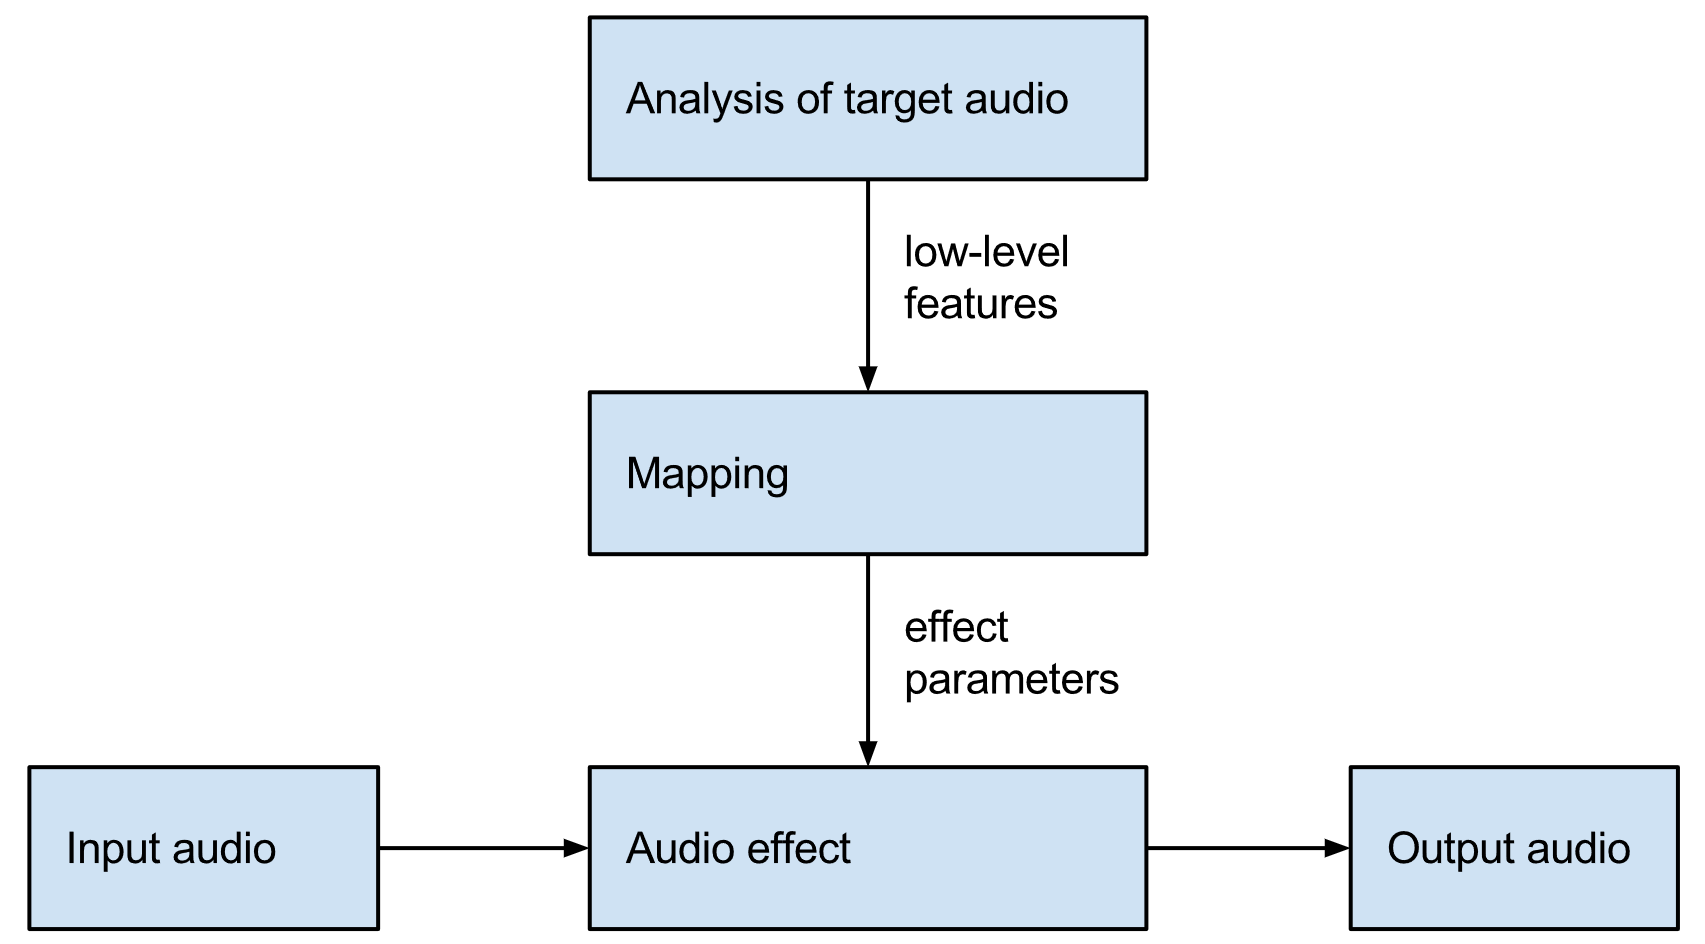
\includegraphics[width=0.6\textwidth]{01_simple_signal}
    \caption{Cross-adaptive audio effect process with two audio streams: input audio and target audio}
    \label{fig:simple_signal}
\end{figure}

In practice, a music performance that uses cross-adaptive audio effects can be a very complex, dynamic system with many signal interactions. However, to limit the scope and complexity of the problem, this project will study signal interactions between only two sounds at a time: an input sound and a target sound. A single audio effect is applied to the input sound. The parameters of this effect are dynamically informed by features from the target audio. The goal of the tool implemented in this project is to make interesting mappings from target audio analysis to audio effect parameters. Brandtsegg (2015) suggested that machine learning can be useful in this context. Generally, for a machine learning problem to be well-defined, a performance measure is needed. A good performance measure would be “how appealing does it sound?”. However, what generally sounds appealing to humans is tacit knowledge and cannot be simply described mathematically. Because there are no good objective measures of what a good cross-adaptive audio effect is, an assumption has been made in this project: If a cross-adaptive audio effect makes features of one sound audible in the other sound, then it is considered interesting. Therefore it has been decided that the objective of the system in this project should be to make the input sound similar to the target sound.

The mapping (figure 1.1) is a function that maps n-dimensional vectors (audio features) to m-dimensional vectors (effect parameters). Artificial neural networks are apt for this, as they can approximate a wide variety of continuous functions (Hornik, 1991). Backpropagation (Werbos, 1982; Lecun, Buttou, Orr, \& Müller, 1998) is an efficient algorithm for training neural networks (i.e. finding a set of useful weights for it), but it requires target values for the output nodes to compute error signals. Since no sets of target values are available for this project, and there is generally no good way of telling exactly how the mapping affects the resulting sound, it makes sense to use evolutionary computation to train the neural networks instead. That is feasible because it is possible to construct a fitness function that returns a score based on how similar two sounds are. All in all, this project is about developing a toolkit that explores evolutionary computation in various ways to evolve artificial neural networks that act as mappings in cross-adaptive audio effects.

As the developed system has many components and deals with lots of numbers in the form of audio features, neural network weights, audio effect parameters, output sounds and fitness values, it’s hard to understand what the system really does. To alleviate this, a significant part of the project has been about developing a comprehensive interactive visualization system as a part of the toolkit. One motivation for this is that one cannot improve the optimization process if one does not know where it fails. It was also made in order to make the toolkit more human-understandable and to make evaluation of results more efficient.

% !TEX encoding = UTF-8 Unicode
%!TEX root = thesis.tex
% !TEX spellcheck = en-US
%%=========================================
\chapter{Background Information}
\label{chapter:background_information}

\section{Genetic Algorithms}
Genetic algorithms \citep{goldberg1989, back1996} are iterative algorithms that can approximate solutions to optimization problems. In such problems, one usually doesn’t know how to construct a good solution, but it is possible to measure how good a solution is. The methods used in genetic algorithms are inspired by Darwin's principle of natural selection. In the algorithm, a population of individuals is simulated through generations of ``life". Each individual is a candidate solution to the optimization problem. The fittest individuals, as determined by a fitness function, are the individuals that are most likely to survive and reproduce (either asexually or sexually). Individuals that are deemed less fit are more likely to die young, and do not get to pass their genes on to future generations. During reproduction, crossover and mutation occurs. Crossover is a genetic operator that combines two parents to produce an offspring. Mutation is a genetic operator that alters an individual slightly. The whole process is roughly illustrated by figure \ref{fig:genetic_algorithm_cycle}.

\begin{figure}[H]
    \centering
    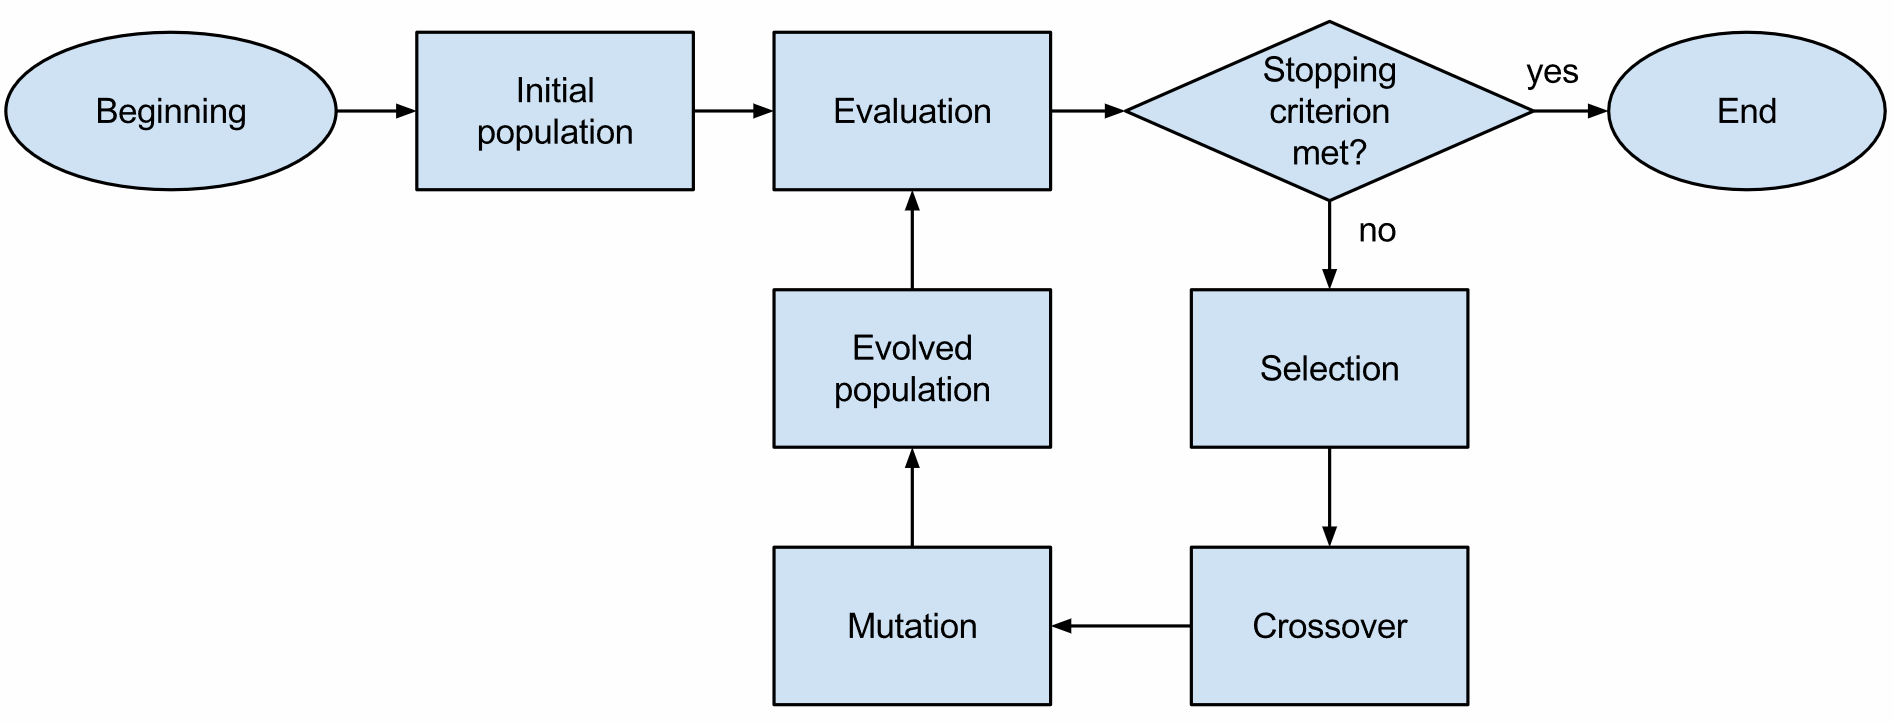
\includegraphics[width=1.0\textwidth]{02_genetic_algorithm_cycle}
    \caption{Genetic algorithm cycle}
    \label{fig:genetic_algorithm_cycle}
\end{figure}

\section{Artificial Neural Networks}
Artificial Neural Networks (ANN) are systems of interconnected ``neurons", or nodes \citep{caudill1987}. A connection from a node A to a different node B means that the activation level of node A influences the activation level of node B based on the numerical weight of the connection. The activation level of a node is calculated by adding up all incoming signals to that node and running that number through the node's activation function. An ANN can be thought of as a function that transforms n-dimensional vectors to m-dimensional vectors. Figure \ref{fig:neural_network} illustrates a simple neural network and the inner workings of one of the nodes.

\begin{figure}[H]
    \centering
    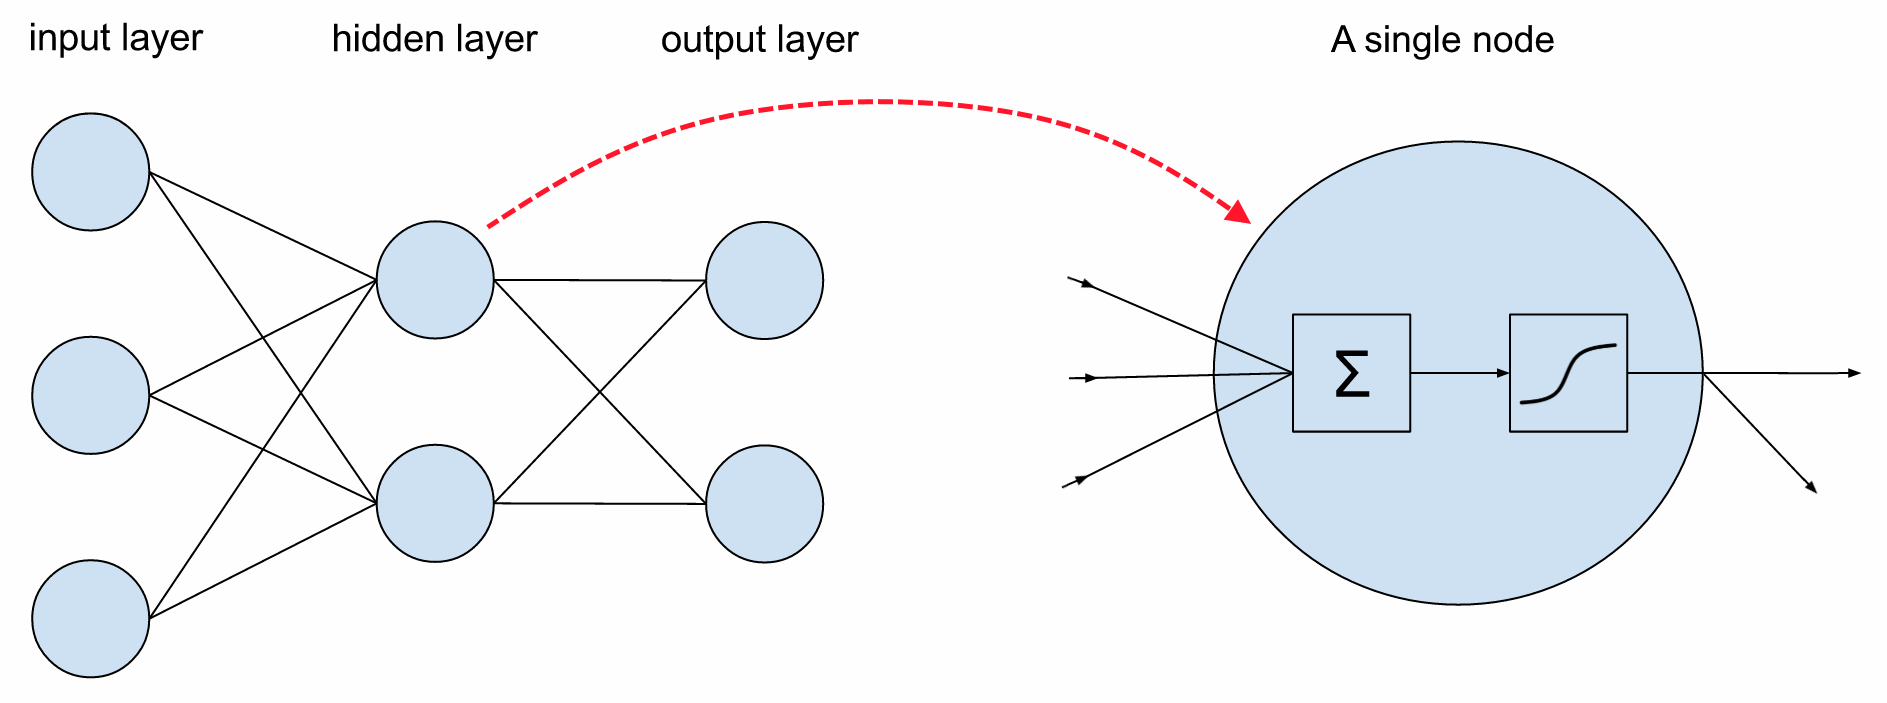
\includegraphics[width=1.0\textwidth]{neural_network}
    \caption{To the left: Illustration of a small neural network with one hidden layer. To the right: Illustration of a hidden node with sigmoid activation function}
    \label{fig:neural_network}
\end{figure}

\section{Neuroevolution}
Neuroevolution is a technique that uses evolutionary algorithms to train artificial neural networks. It differs from supervised learning algorithms such as backpropagation in that it does not require a set of correct input-output pairs. Instead, only a performance measure (fitness function) is needed.

\section{NeuroEvolution of Augmenting Topologies (NEAT)}
NEAT \citep{stanley2002} is a neuroevolution technique that evolves neural networks with genetic algorithms. Not only the weights of the ANN are evolved, but also the structure. The NEAT approach begins with a feed-forward approach with input nodes and output nodes that are fully connected. The ANN can then grow larger by having nodes and links added to it. NEAT can also remove nodes and links.

\iffalse
TODO:
Competing conventions
Species
Genotype (list of nodes, list of connections)
Phenotype
Crossover
Interspecies crossover
Dynamic compatibility
Min species
Max species
Aging species
Innovations
Young age fitness boost
Species stagnation
Competitive coevolution stagnation
Kill worst species each 15 generations
Survival rate
Elitism
Tournament selection
Sexual vs asexual reproduction?
Mutation operations
\fi

\section{Multi-Objective Evolutionary Algorithms}
As real-life problems often have more than one objective, there is a need for ways to deal with multiple objectives effectively. A multi-objective evolutionary algorithm (MOEA) is an algorithm for solving mathematical optimization problems involving more than one objective function to be optimized simultaneously \citep{veldhuizen2000}. One well-known algorithm of this kind is Nondominated Sorting Genetic Algorithm II (NSGA-II) \citep{nsga2}. In this algorithm, the performance measure is based primarily on rank and secondarily on crowding distance. Rank is calculated by running the fast non-dominated sort algorithm. This algorithms assigns a rank to each individual. If the rank of individual A is better than the rank of another individual B, it means that A dominates B. Individual A dominates B if both the following conditions are true:

\begin{itemize}  
\item The solution A is no worse than B in all objectives.
\item The solution A is strictly better than B in at least one objective.
\end{itemize}

Crowding distance is a way to measure how crowded the search space around the individual is. Crowding distance is quantified by forming a cuboid with the nearest neighbours as vertices, and then taking the average of the side lengths of the cuboid. Large crowding distances are encouraged because it preserves diversity in the population \citep{nsga2}.

\section{Audio Feature Extraction Tools}
Audio feature extraction is the process of computing a compact numerical representation that can be used to characterize a segment of audio. Low-level features such as spectral centroid and Mel-Frequency Cepstral Coefficients (MFCC) \citep{mermelstein1976, logan2000} are computed directly from the audio signal, frame by frame. A frame is a slice of audio and can consist of for example 1024 samples. In an audio signal with sampling rate 44.1 kHz, the duration of such a frame would be approximately 23 ms.

Audio features can be used in many different ways, such as music information retrieval and musical genre classification. In this project, they are used for similarity measures and for controlling the parameters of audio effects. Four audio feature extraction tools were used in this project: Aubio \citep{brossier2003aubio}, Essentia \citep{bogdanov2013essentia}, LibXtract \citep{bullock2007libxtract} and Csound \citep{csound}.

\section{Audio Effects}
Audio effects are processing techniques that alter audio so it sounds different. The following subsections describe the audio effects used in this project.

\subsection{Modified Hyperbolic Tangent}
Modified hyperbolic tangent is a waveshaping function that can model the characteristics of analog distortion, and especially tube distortion \citep{mtanh}. Modified hyperbolic tangent differs from hyperbolic tangent in that one can model the positive and the negative slopes differently. This distortion effect makes the sound ``fuzzier" by adding harmonic components. Figure \ref{fig:modified_hyperbolic_tangent_waveform_and_spectrum} illustrates an example of this.

$$\text{mtanh}(x)=\frac{e^{ax}-e^{-bx}}{e^{cx}+e^{-dx}}$$

\begin{figure}[H]
    \centering
    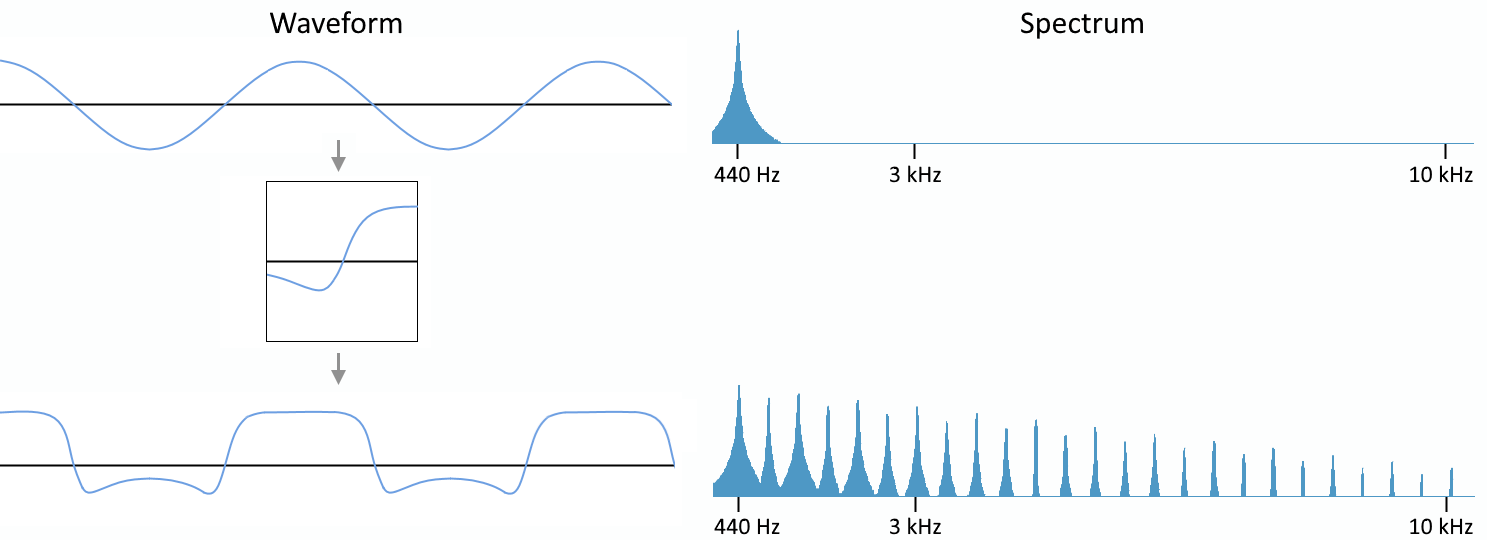
\includegraphics[width=1.0\textwidth]{modified_hyperbolic_tangent_waveform_and_spectrum}
    \caption{Harmonic frequency components are added to a 440 Hz sine wave by applying a modified hyperbolic tangent function}
    \label{fig:modified_hyperbolic_tangent_waveform_and_spectrum}
\end{figure}

\subsection{Low-Pass Filter}
A low-pass filter attenuates high frequencies and retains low frequencies unchanged \citep{dodge_jerse_1997}. It can be used to make a sound ``darker" or ``smoother" in timbre. A resonant low-pass filter is a low-pass filter that has a peak in the response curve at the cutoff frequency, as illustrated by figure \ref{fig:low_pass_filter}. This quality can be used to boost a single tone in a sound with a rich frequency spectrum. The width of the resonant peak is described by a parameter called Q. As Q increases, the resonance becomes more pronounced.

\begin{figure}[H]
    \centering
    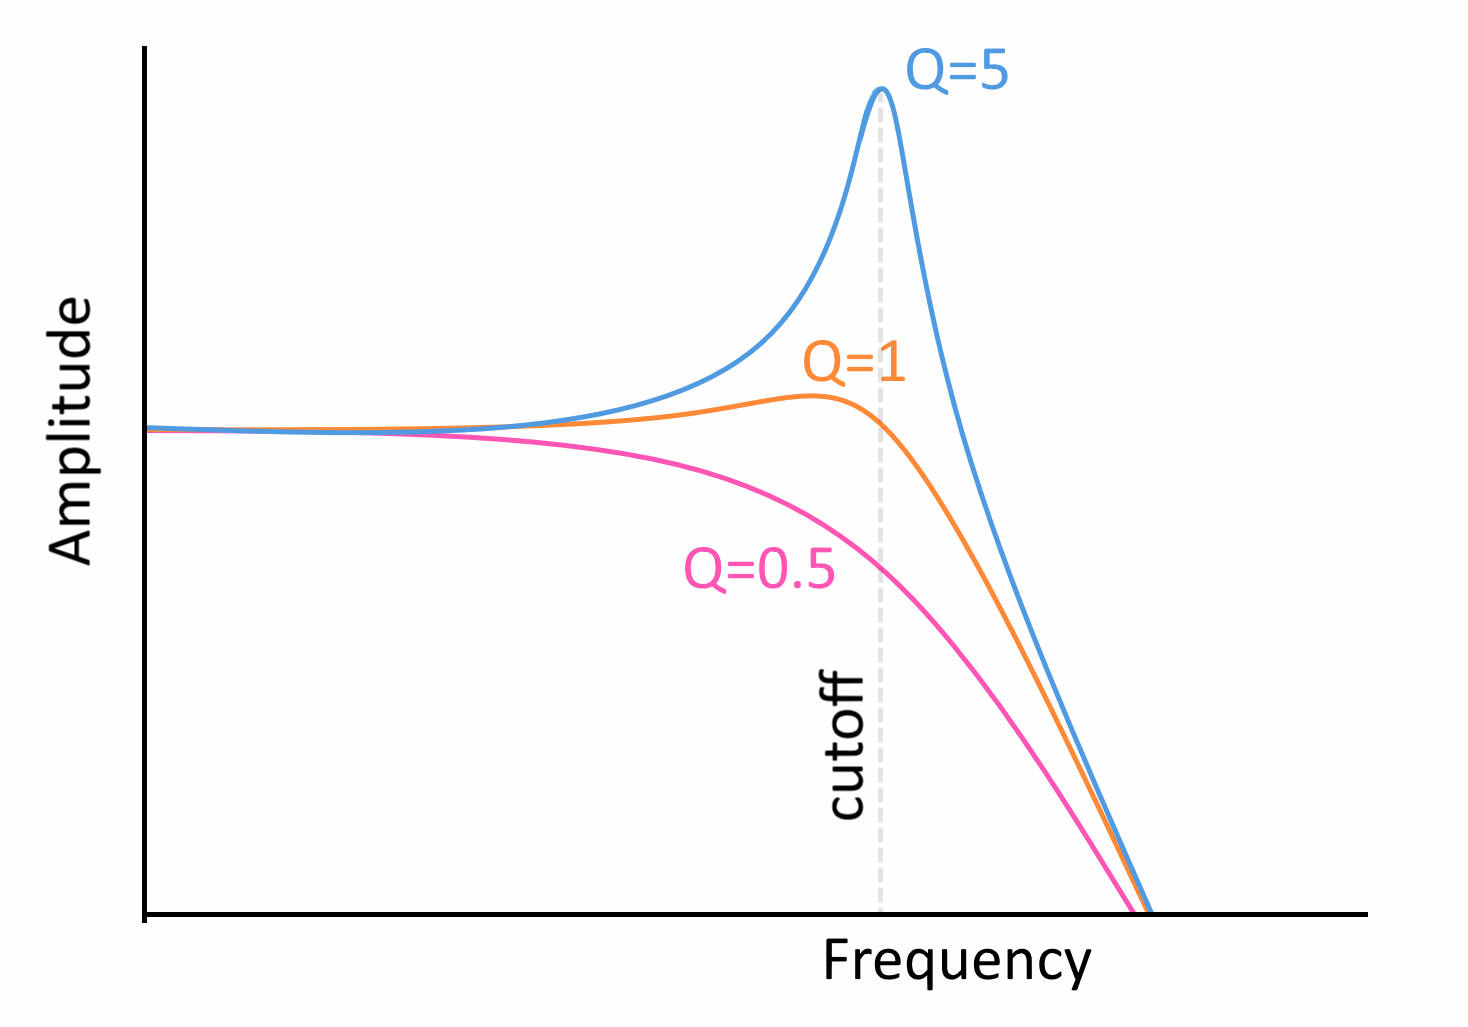
\includegraphics[width=0.5\textwidth]{05_low_pass_filter}
    \caption{Frequency response of a resonant low-pass filter with various Q values}
    \label{fig:low_pass_filter}
\end{figure}

\subsection{Band-Pass Filter}
A band-pass filter rejects frequencies outside a given range \citep{dodge_jerse_1997}. This filter has two parameters. Center frequency (denoted by $f_0$ in figure \ref{fig:bandpass}) defines the center of the frequency range. Bandwidth (denoted by $B$ in figure \ref{fig:bandpass}) defines how broad or narrow the frequency range is.

\begin{figure}[H]
    \centering
    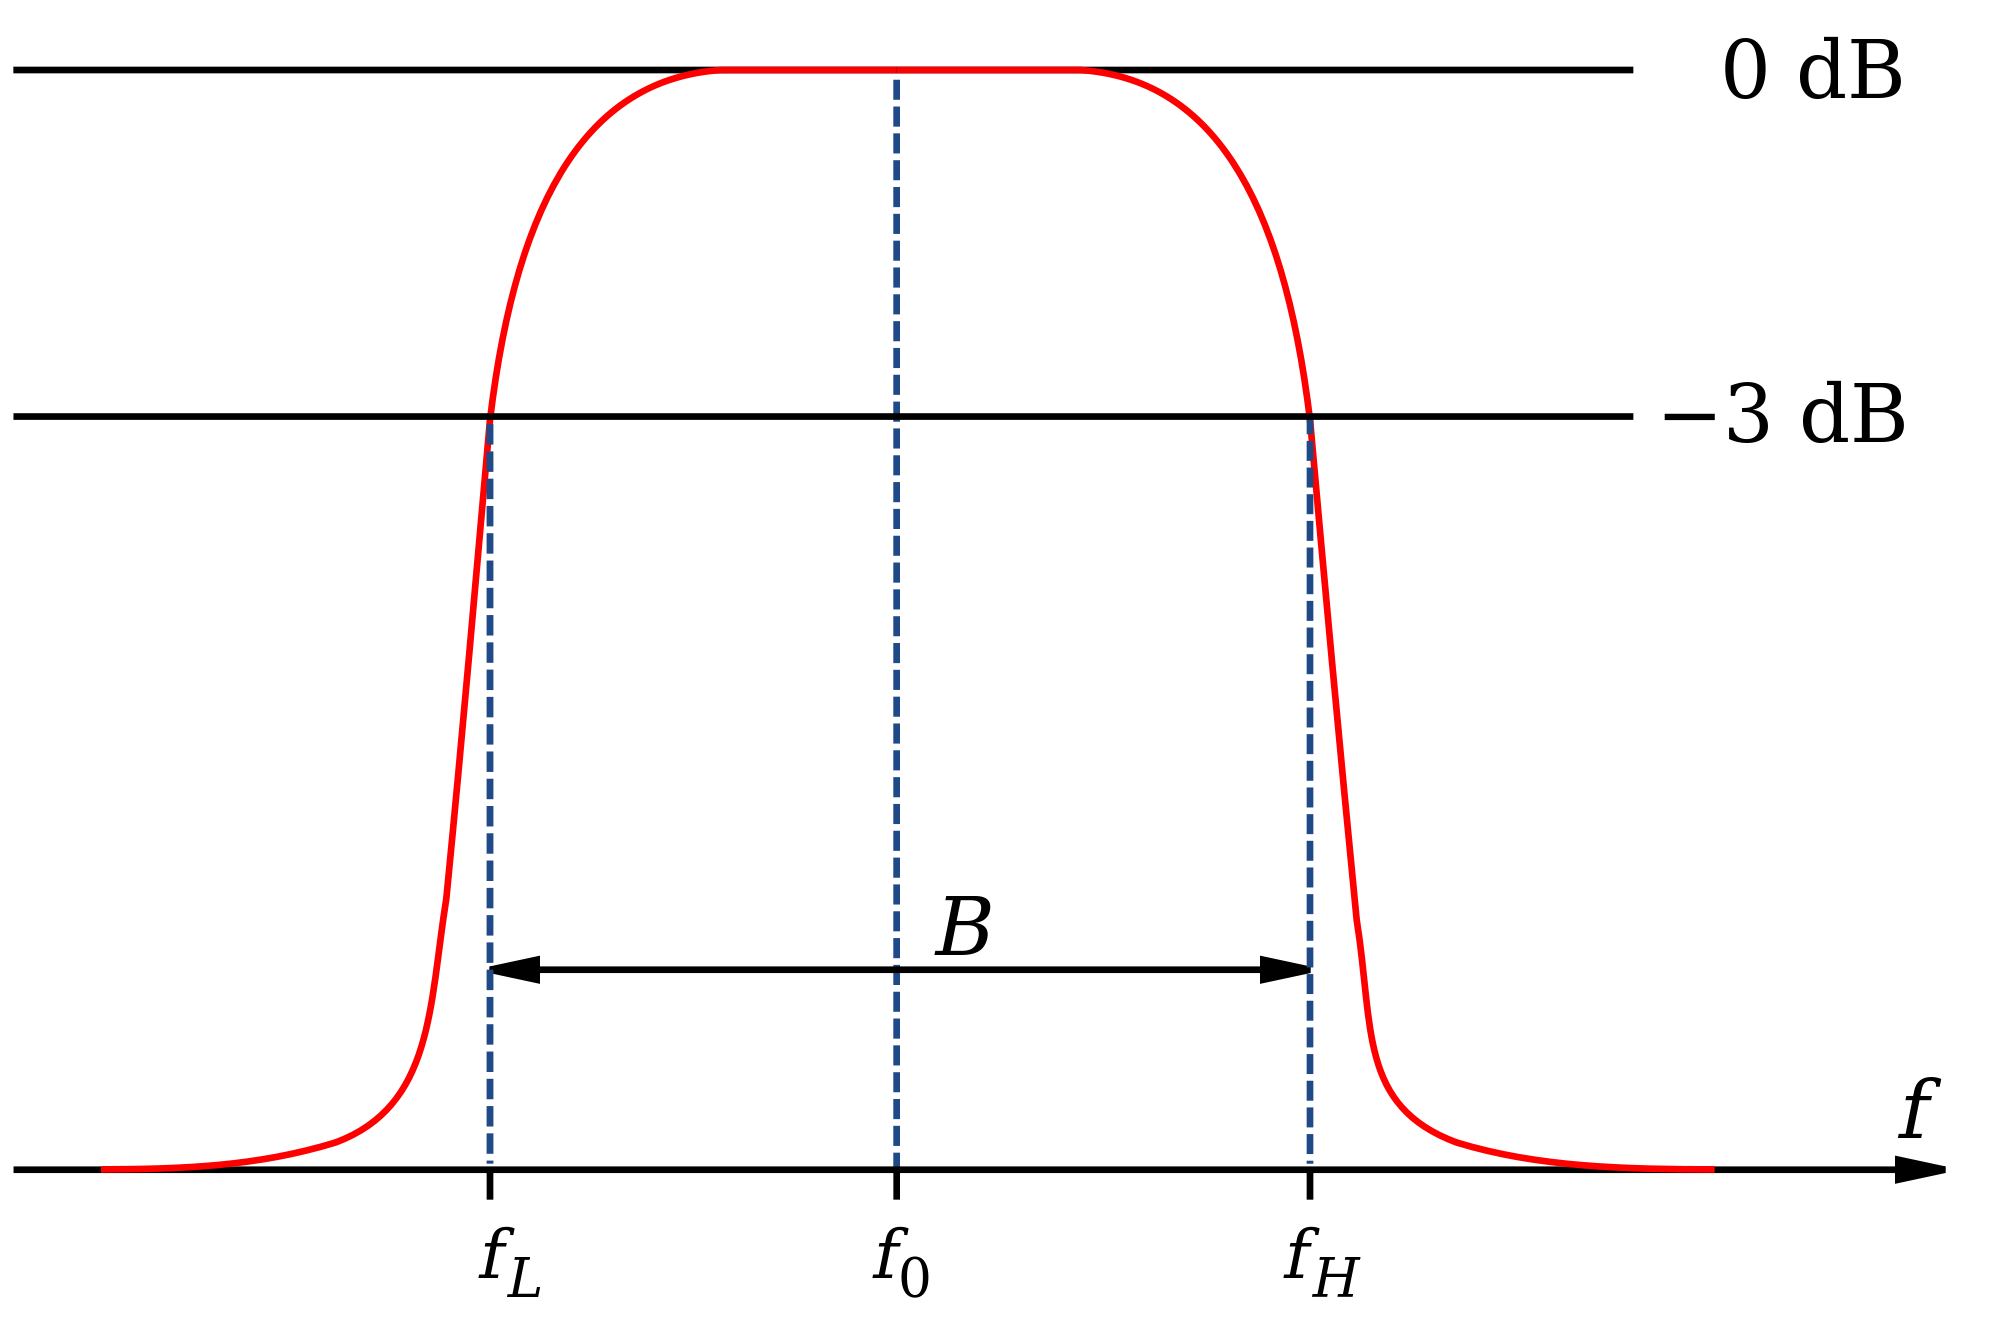
\includegraphics[width=0.5\textwidth]{bandpass}
    \caption{A diagram that illustrates the frequency response of a band-pass filter and defines its bandwidth}
    \label{fig:bandpass}
\end{figure}

\subsection{Amplitude Modulation}
The amplitude modulation effect multiplies the sound signal with a unipolar sine wave that oscillates between 0 and 1. When the frequency of the sine wave is low (\textless~20 Hz), one can hear that the amplitude is being brought up and down, as in tremolo \citep{serafin2007}. With higher frequencies there is instead an effect on the timbre of the sound. The modulator generates a set of frequency sidebands, as illustrated in figure \ref{fig:am_sidebands}

\begin{figure}[H]
    \centering
    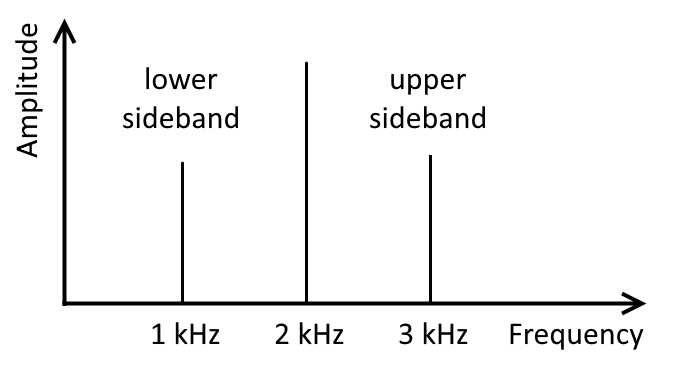
\includegraphics[width=0.5\textwidth]{am_sidebands}
    \caption{Frequency spectrum plot of a 2 kHz sine wave modulated with a 1 kHz unipolar sine wave}
    \label{fig:am_sidebands}
\end{figure}

\subsection{Bit Reduction}
The bit reduction effect reduces the number of bits used to represent a sample \citep{bitreduction}. Each sample amplitude value is rounded to a number of discrete steps. This introduces a particular kind of distortion, also called quantization noise.

\begin{figure}[H]
    \centering
    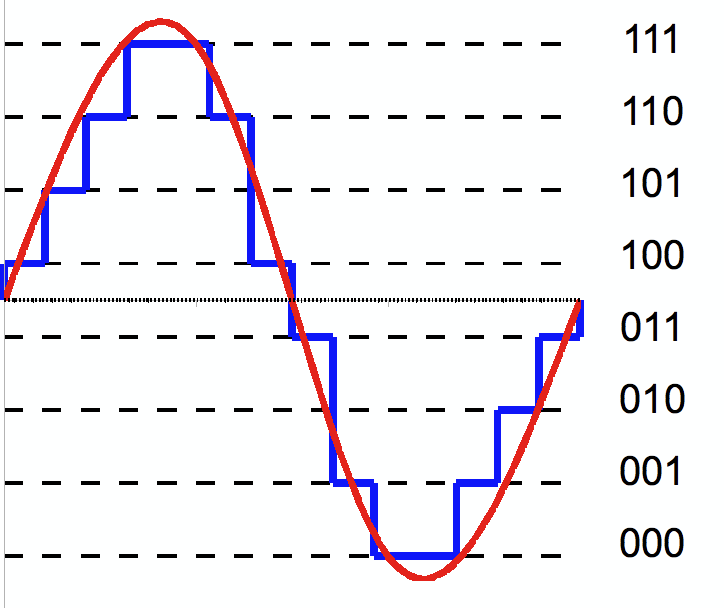
\includegraphics[width=0.3\textwidth]{bit_reduction}
    \caption{A high fidelity sine wave quantized to 3 bits per sample. \textit{By Hyacinth, CC BY-SA 3.0, \url{https://commons.wikimedia.org/w/index.php?curid=30716342}}}
    \label{fig:bit_reduction}
\end{figure}

\subsection{Chorus}
The chorus effect delays the input signal by a short \textit{delay time} (usually in the range 20-50~ms) and mixes it with the dry input signal \citep{chorus}. The \textit{delay time} is variable and usually controlled by a Low-Frequency Oscillator (LFO), as illustrated by figure \ref{fig:chorus}. This may create an impression of multiple voices playing or singing the same thing.

\begin{figure}[H]
    \centering
    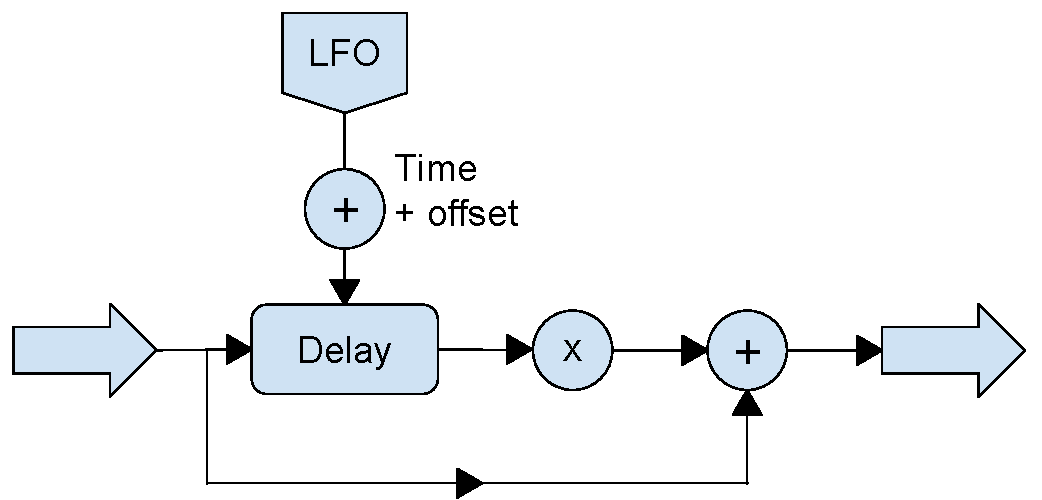
\includegraphics[width=0.5\textwidth]{chorus}
    \caption{Signal flow in a chorus effect}
    \label{fig:chorus}
\end{figure}


\section{Audio Processing Tools}
Audio processing is the alteration of audio signals, typically through audio effects. One popular audio processing tool is Csound \citep{csound}. This is both an audio programming language and a program that runs Csound code. The Csound program takes in a text file of code. This code is executed by the Csound program. The output is sound that is directed to either an audio interface (live) or to a file (non-real-time processing). Csound is used by musicians and composers, typically in experimental electroacoustic music. Traditionally, it has been an offline tool, due to lack of computational power. Today, computational power is sufficient for Csound to run in real-time, so it can be used in live settings such as concerts and sound installations. Csound can not only run on desktop computers, but can also be used as audio processing engine in mobile applications for the operating systems Android and iOS.

\section{Specialization Project}
This master's thesis is a continuation of the author's specialization project. The preliminary experiments in the specialization project were found to be successful. This led to a published paper in the proceedings of the 2nd AES Workshop on Intelligent Music Production\footnote{\url{http://www.aes-uk.org/forthcoming-meetings/wimp2/\#proceedings}}. This paper is included in appendix \ref{appendix:jordal_paper}. The author also presented his findings in a 15-minute talk at this event.

The following subsections will summarize some of the main areas of study in the experiments in the specialization project.

\subsection{Output Activation Functions}
Three different output activation functions (used in the output nodes of the neural networks) were compared. Sigmoid was found to be better than linear and sine in most cases (see figure \ref{fig:output_activation_functions_avg}).

\begin{figure}[H]
    \centering
    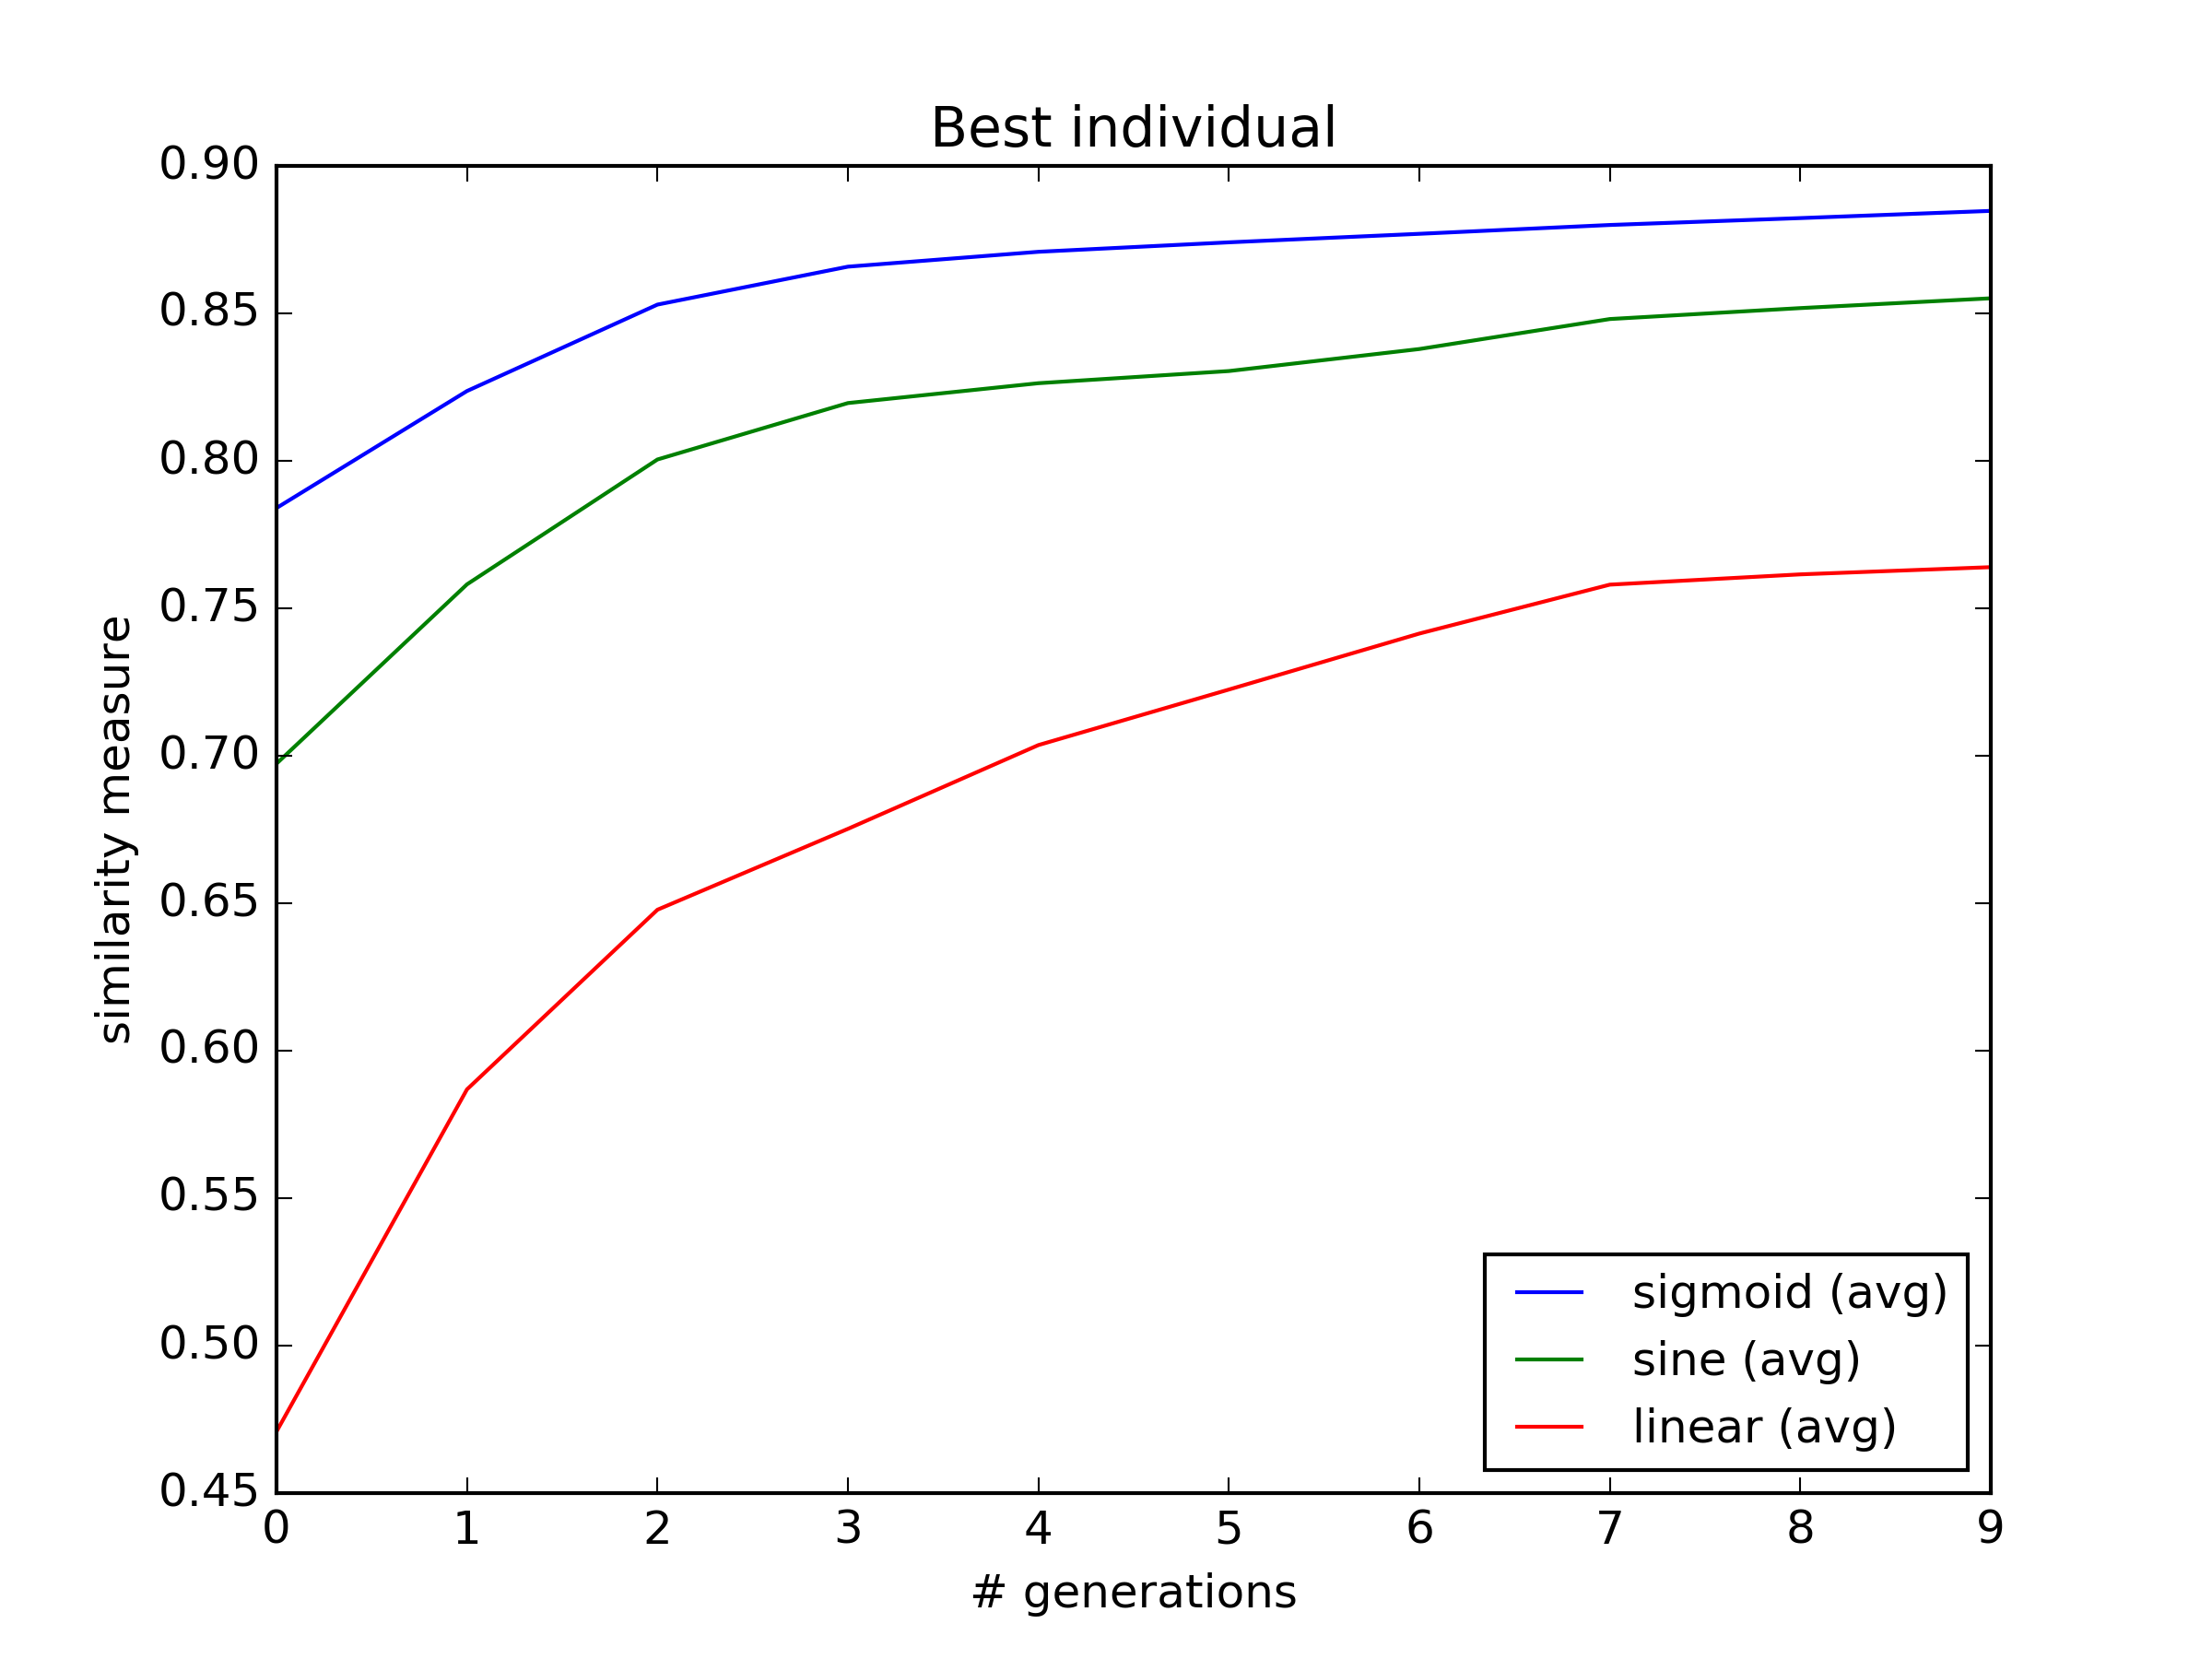
\includegraphics[width=0.85\textwidth]{output_activation_functions_avg}
    \caption{Average fitness over 20 runs}
    \label{fig:output_activation_functions_avg}
\end{figure}

\subsection{Fitness Functions}
Five fitness functions were compared. Figure \ref{fig:fitness_functions_avg} shows how well they scored on average on the similarity measure (local similarity).

\subsubsection{Local Similarity}
The local similarity fitness function is based on the average euclidean distance between the feature vector of the target sound and the output sound in the k frames of the two sounds.

\begin{verbatim}
Function LOCAL_SIMILARITY(target, individual):
    total_euclidean_distance = 0
    for each k in range(num_frames):
        A = target.get_feature_vector(k)
        C = individual.get_feature_vector(k)
        total_euclidean_distance += EUCLIDEAN_DISTANCE(A, C)
    avg_euclidean_distance = total_euclidean_distance / num_frames
    return 1 / (1 + avg_euclidean distance)
\end{verbatim}

where \texttt{EUCLIDEAN\_DISTANCE} is $d(p,q)=\sqrt{(q_1-p_1)^2+(q_2-p_2)+...+(q_n-p_n)^2}$

\subsubsection{Multi-Objective Optimization}
This fitness function is inspired by NSGA-II \citep{nsga2}. It incorporates two measures: rank and crowding distance. These are concepts taken directly from the NSGA-II paper, and they are then used in a math expression that satisfies these two constraints that are used in NSGA-II:

\begin{itemize}
\item $\text{rank}(A) > \text{rank}(B) \implies \text{fitness}(A) > \text{fitness}(B)$
\item $\text{rank}(A) = \text{rank}(B), \text{CD}(A) > \text{CD}(B) \implies \text{fitness}(A) > \text{fitness}(B)$
\\ where CD stands for crowding distance
\end{itemize}

The ranks of the individual are calculated by doing non-dominated sort. Crowding distance is computed between individuals in a given rank. The multi objective fitness function works like this:

\begin{Verbatim}[fontsize=\small]
Function MULTI_OBJECTIVE(target, individuals):
    for individual in individuals:
        CALCULATE_OBJECTIVES(individual, target)
    fronts = FAST_NON_DOMINATED_SORT(individuals)
    for rank in fronts:
        CALCULATE_CROWDING_DISTANCE(fronts[rank])  # assigns individual.crowding_distance
        for individual in fronts[rank]:
            individual.fitness = 1.0 / (rank + (0.5 / (1.0 + individual.crowding_distance)))

Function CALCULATE_OBJECTIVES(individual, target):
    individual.objectives = {}
    for feature in similarity_features:
        individual.objectives[feature] = EUCLIDEAN_DISTANCE(
                                             target.analysis[feature],
                                             output.analysis[feature])
\end{Verbatim}

Pseudocode for \texttt{FAST\_NON\_DOMINATED\_SORT} and \texttt{CALCULATE\_CROWDING\_DISTANCE} can be found in the NSGA-II paper \citep{nsga2}.

\subsubsection{Hybrid}
While NSGA-II is good at optimizing for non-dominated individuals, these individuals may be extreme tradeoffs and therefore not necessarily feasible solutions in practice. In order to reward good tradeoffs more, the author developed the hybrid fitness function. This fitness function returns the average of \texttt{MULTI\_OBJECTIVE} and \texttt{LOCAL\_SIMILARITY}.

\subsubsection{Novelty Search}
Novelty search \citep{lehman2008} ignores the objective and optimizes for novelty instead. The reason that this may work well is that in some problems the intermediate steps to the goal do not resemble the goal itself. When it comes to implementation, MultiNEAT has novelty search built-in, but Python bindings for it are missing, so the author could not use it in his Python application. However, novelty search can be implemented on top of most evolutionary algorithms, by using a fitness function that rewards novelty \citep{noveltysearchwebsite}, so that is what the author did. First, each individual needs to be represented as a vector that describes its characteristics. This vector is constructed by concatenating all audio feature series of the individual. The implemented fitness function assigns high fitness values to the individuals that have long euclidean distances from the 3 nearest neighbours, where the neighbours are individuals that have been evaluated earlier. The very first population gets random fitness values, because there are no earlier individuals to measure distance from.

\subsubsection{Mixed}
This fitness function is simple: For each generation, one of the following fitness functions is chosen randomly and applied: local similarity, multi-objective, hybrid, novelty. The idea behind this fitness function is to create a dynamic fitness landscape, where the individuals that get good scores from all fitness functions have the greatest chance of survival over time.

\begin{figure}[H]
    \centering
    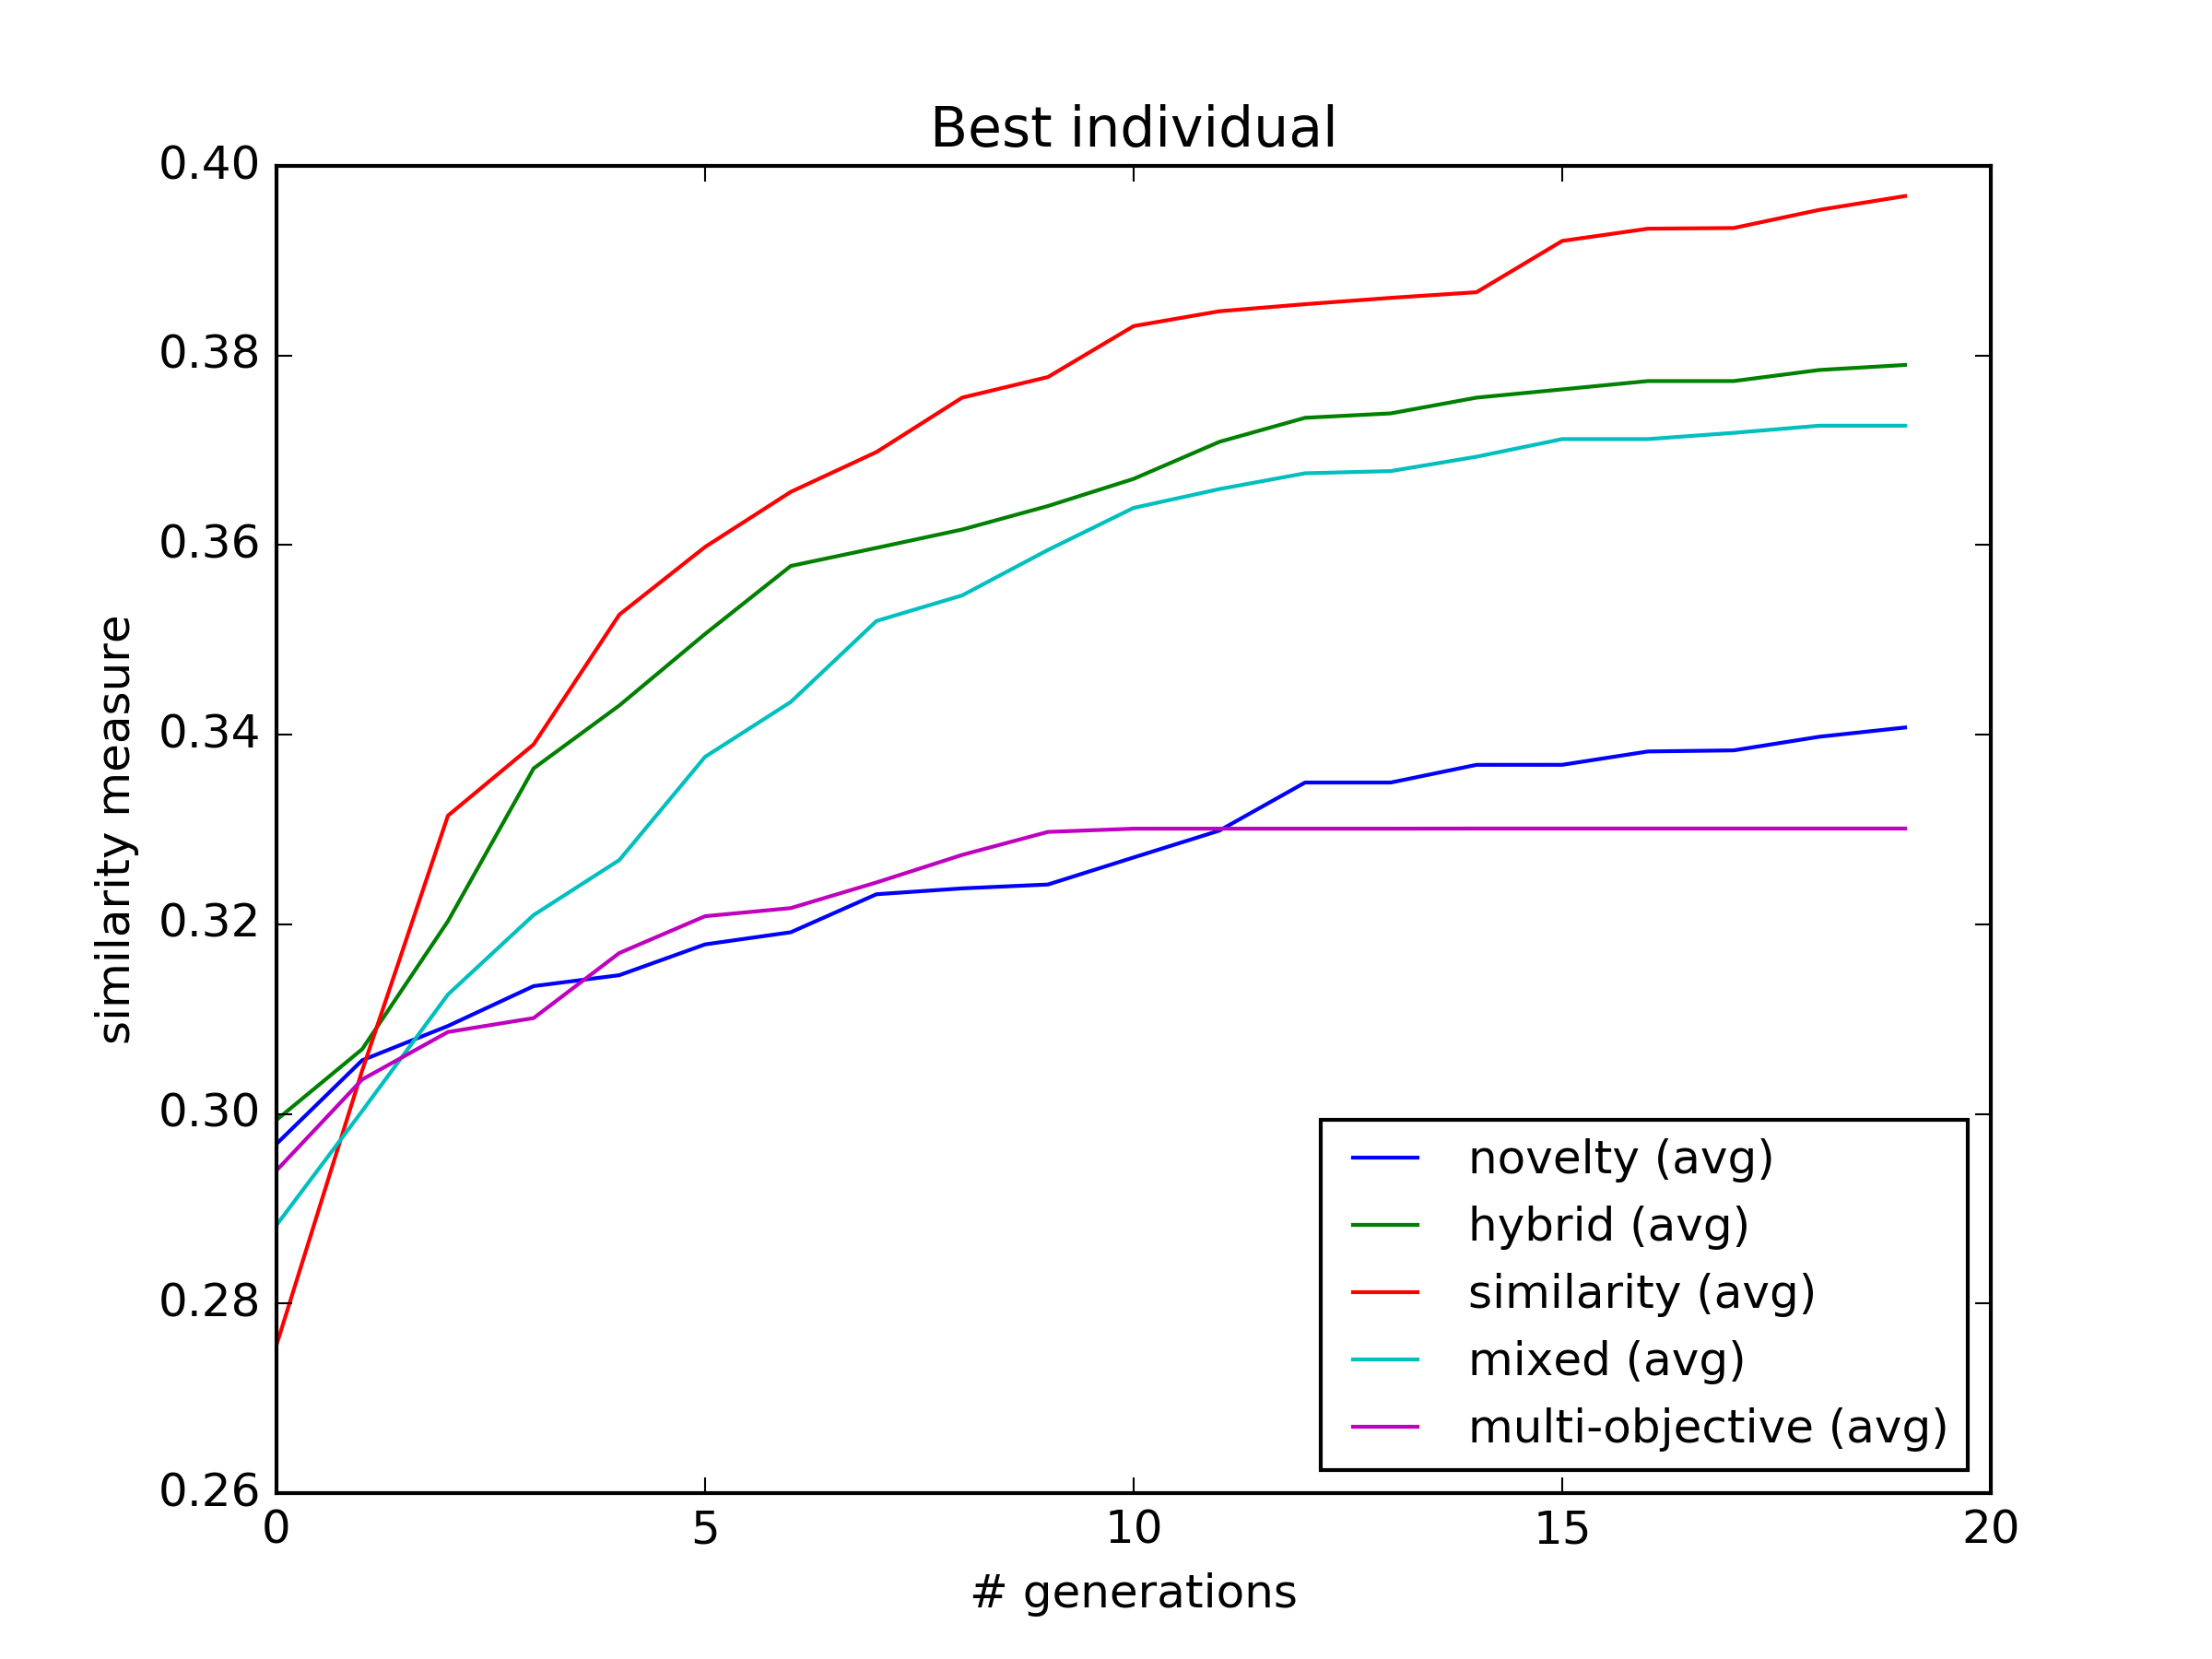
\includegraphics[width=0.85\textwidth]{fitness_functions_avg}
    \caption{Best individual on average over 20 runs, with 20 generations for each run}
    \label{fig:fitness_functions_avg}
\end{figure}

\subsection{Automatic Feature Selection}
When dealing with high-dimensional input data, the number of weights in a fully connected neural network becomes quite large. Clean and useful combinations of all the input signals can be hard to evolve. To deal with this situation, one can use Feature Selective NeuroEvolution of Augmenting Topologies (FS-NEAT) \citep{whiteson2005}. This NEAT variation starts with just a few connections and gradually adds/removes connections.

In an experiment with noise for input sound and a sine sweep for output sound, FS-NEAT was found to perform better than classic NEAT. This experiment had 68 audio features as input. Classic NEAT would typically evolve a very noisy parameter control, so the output sounds became glitchy and not very musically interesting. FS-NEAT has been found to deal with the high-dimensional input more effectively, as it selected only a few of the audio features that were useful for getting high fitness values. Figure \ref{fig:neat_vs_fs_neat_avg_max} shows fitness values with NEAT and FS-NEAT in the described experiment.

\begin{figure}[H]
    \centering
    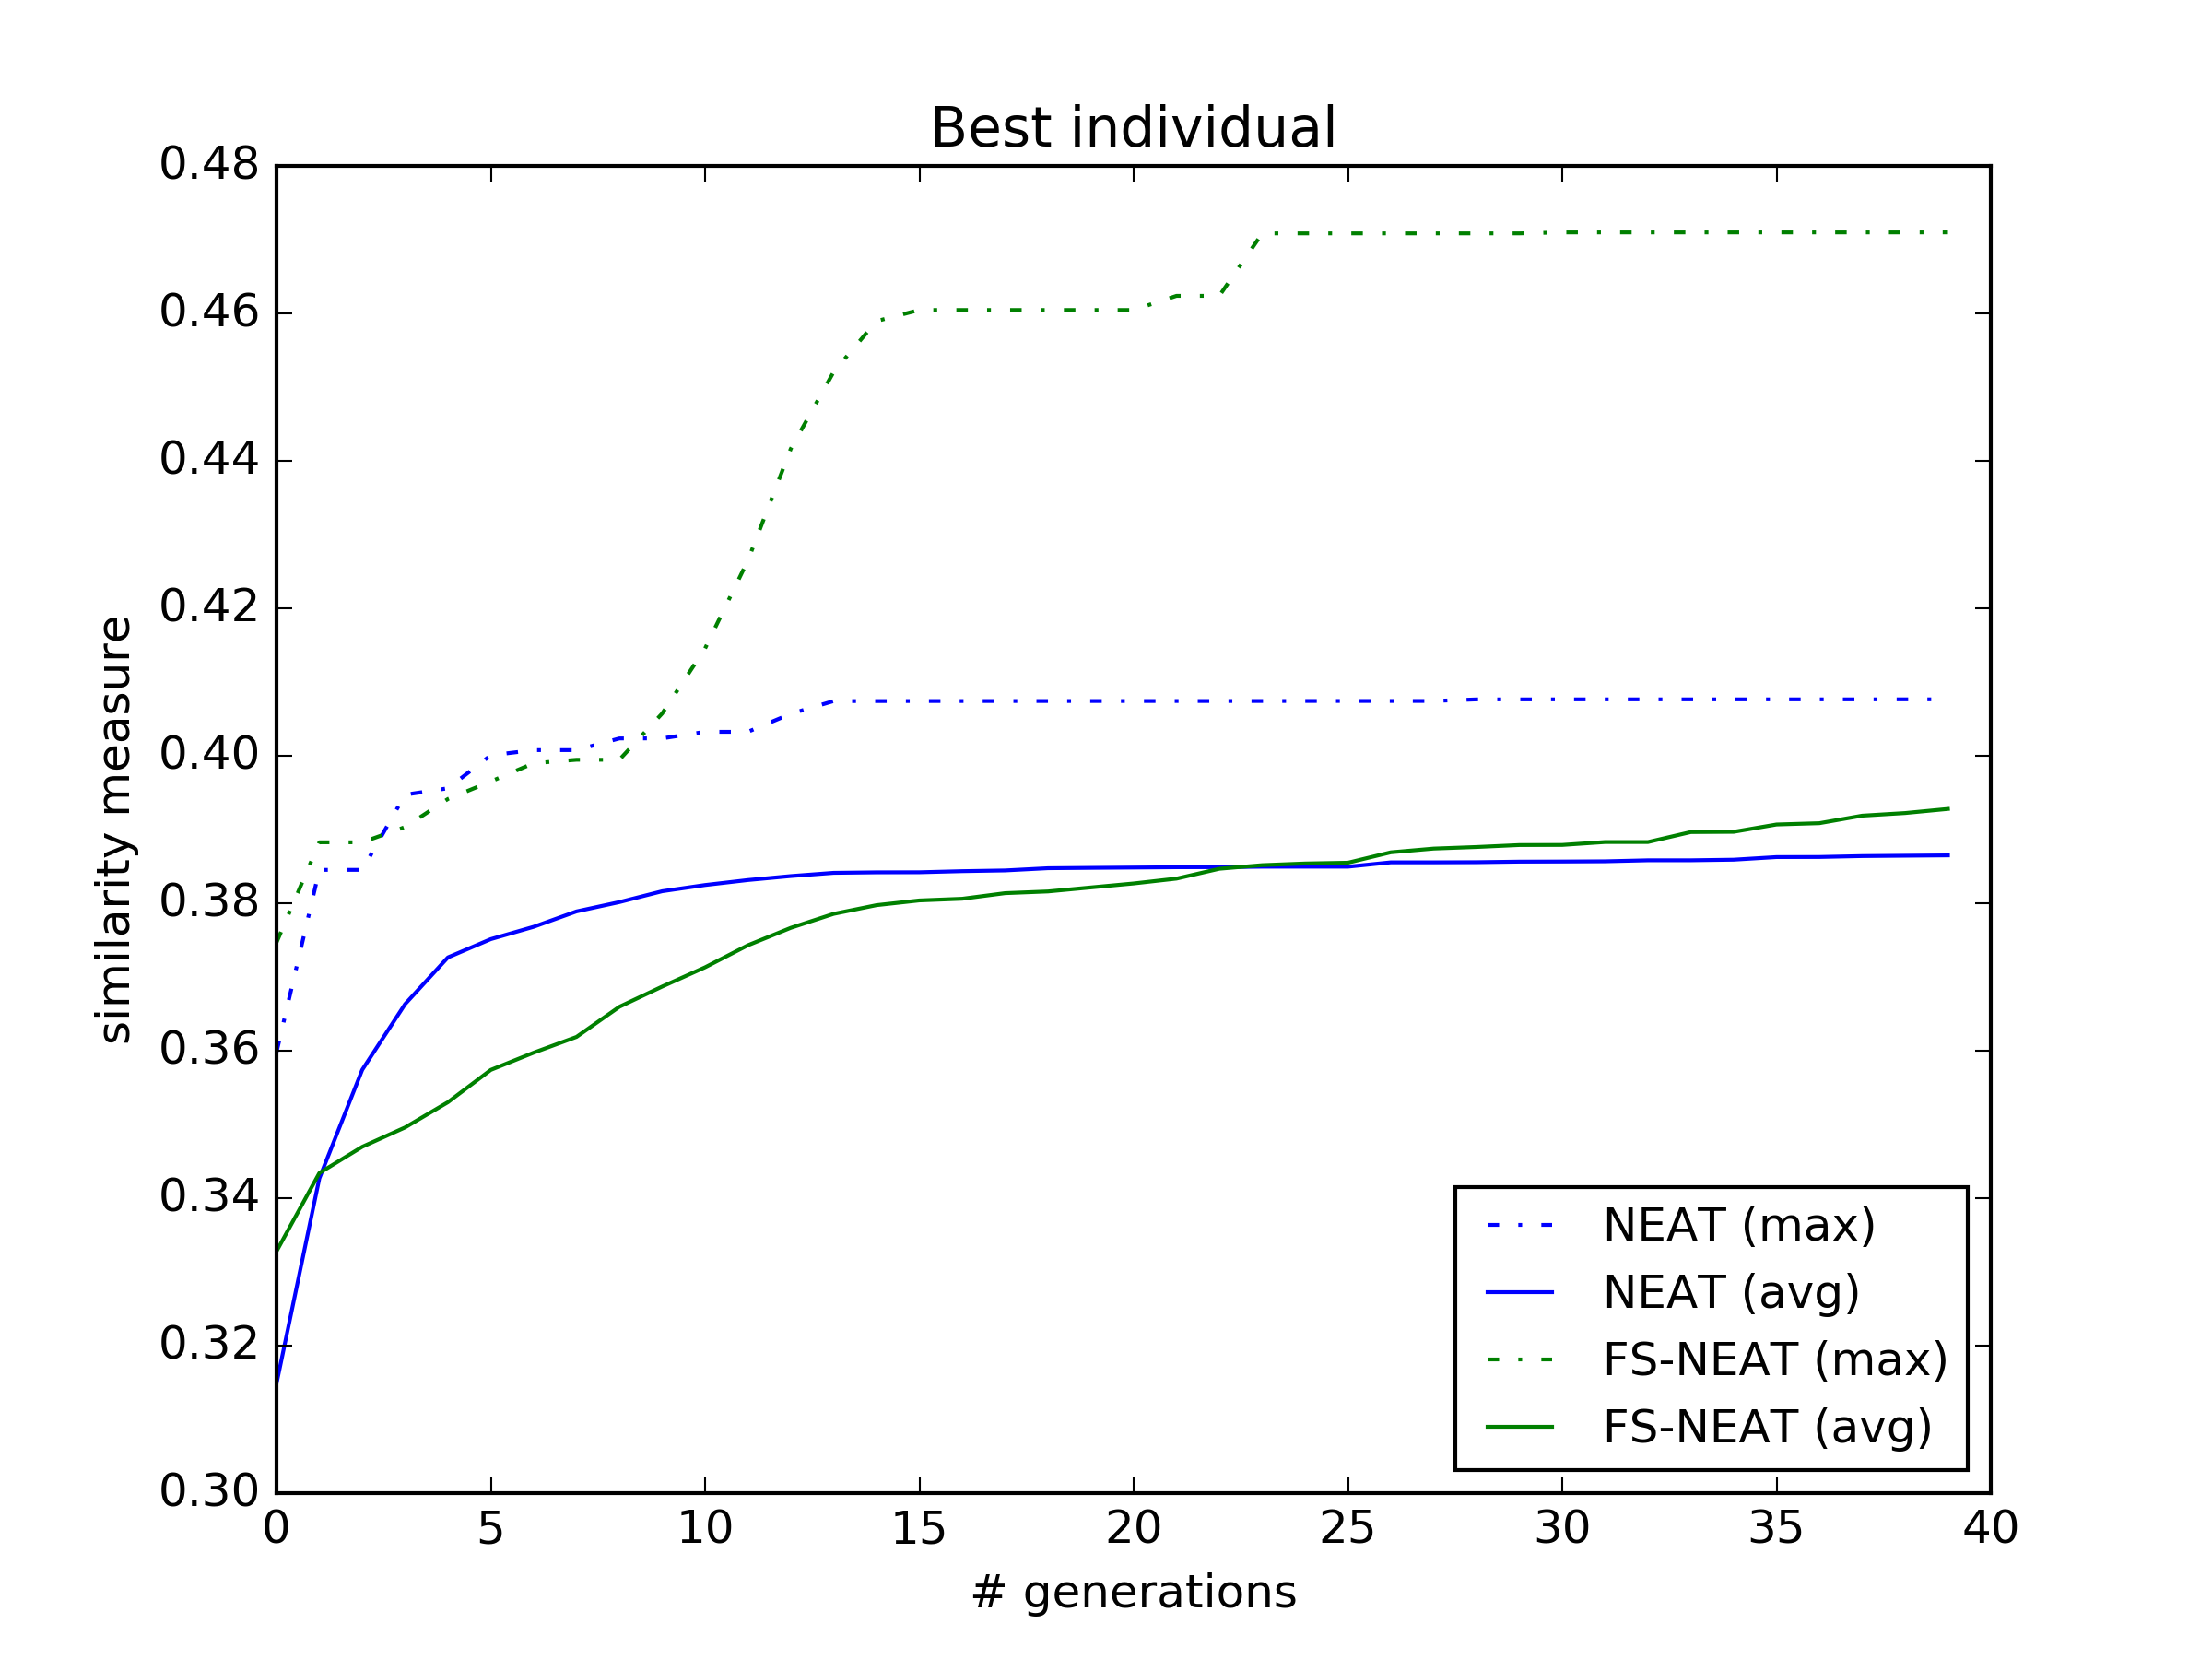
\includegraphics[width=0.85\textwidth]{neat_vs_fs_neat_avg_max}
    \caption{Fitness values in runs with NEAT and FS-NEAT, aggregated from 20 runs with each configuration.}
    \label{fig:neat_vs_fs_neat_avg_max}
\end{figure}




% !TEX encoding = UTF-8 Unicode
%!TEX root = thesis.tex
% !TEX spellcheck = en-US
%%=========================================
\chapter{Methods and implementation}

\section{Evolving neural networks}
There are several ways to map sound analysis to effect parameters. The initial idea was a modulation matrix, where each effect parameter becomes a linear combination of the audio features. This idea was quickly iterated upon. Why not use an artificial neural network? An artificial neural network can do the same as a modulation matrix (when the ANN has linear activation functions and no hidden layers), but it can also do more. A neural network can have hidden nodes with various activation functions, which makes more complex signal interactions possible. This widens the scope, and allows for learning higher-level features, such as “the snare and the bass drum are hit simultaneously”.

NEAT (Stanley \& Miikkulainen, 2002) is suggested as a technique for evolving neural networks. This is a technique which evolves not only the weights of the neural network, but also the topology, i.e. the number of nodes and the connections between the nodes. HyperNEAT, a technique that is based on NEAT, has been used with great success in a project called Picbreeder (Secretan et al., 2008) and later with some success in a project called SoundBreeder (Ye \& Chen, 2014). The purpose of those projects were to evolve visually and aurally appealing art, respectively. Since both those two projects and this project are within the field of creative computation, the hypothesis is that NEAT or HyperNEAT will work well in this project.

\section{Implementation}
Csound has been selected to be the audio processing tool in this project. Since Csound interoperates nicely with Python, and Python is a popular language for artificial intelligence (AI) applications, that was the language of choice for the neuroevolution application. Further, it has been decided that the application should be written in a style compatible with both Python 2 and 3, for the sake of compatibility with various Python libraries. Also, it should work on both Windows and Ubuntu. This way, experiments can not only run on Windows desktop computers, but also on Ubuntu instances in the cloud. The most important dependency is MultiNEAT (Chervenski \& Ryan, n.d.), which is one of Kenneth Stanley’s recommended neuroevolution libraries (Stanley, n.d.). It features several neuroevolution algorithms, including NEAT, FS-NEAT and HyperNEAT. It is written in C++, but it has Python bindings, so it is fit for this project. Further, the audio features extraction tools selected for this project are Aubio, Essentia and LibXtract, which are all free open source software written in a compiled language. A link to the author’s implementation of the toolkit, which is open source, is included in appendix A. A complete list of dependencies is included in appendix B.

\subsection{Performance}
A. Eldhuset has previously implemented a program that uses Csound in signal interaction experiments with genetic algorithms. He concluded that his implementation was slow, taking around 5 seconds per individual (Eldhuset, 2015). Hence an experiment with a population size of 20 and 20 generations would take approximately half an hour. The author has analyzed the weaknesses of Eldhuset's approach and come up with a number of techniques to alleviate performance issues:

\begin{itemize}  
\item Use a templating engine to generate Csound files. It writes csound code to different files, one for each individual in the population. This allows many Csound instances to be run in parallel.
\item While a Csound instance runs, it does not have to communicate with another program (a host) via an API. All data needed for the run, including effect parameter values over time, are included inside the csd file
\item Use dedicated, compiled audio feature extraction tools such as Aubio instead of Csound for audio feature extraction
\item Use the standard streams (stdout) instead of file I/O in audio feature extractors that support this
\item Let the host program, Csound and audio feature extractors write files to a RAM disk to avoid slow disk I/O activity
\item Use the concept of pipelining to shorten critical paths and enable more parallelism
\item Sensible handling of duplicate individuals: when two or more individuals are equal (i.e. their neural networks are equal), evaluate only one of them, and apply the same result to the identical individuals
\end{itemize}

Incorporating all these techniques, the author's implementation spends around 0.11 seconds on average per individual, given that the dist\_lpf effect and the aubio mfcc analyzer is used, the duration of the input sound is 7 seconds, and that the program is run on a modern, high-end laptop with two CPU cores. Hence an experiment with population size 20 and 20 generations may take approximately half a minute.

\subsection{Neuroevolution routine}
The neuroevolution program is called from the command line, with a number of arguments for configuring the experiment. The program then performs roughly these steps:

\begin{enumerate}  
\item Check sanity of arguments
\item Analyze input sound file and target sound file
\item Initialize a population
\item For each generation, evaluate all individuals, write their data to json files and then advance to the next generation
\end{enumerate}

The evaluation of an individual involves several operations:

\begin{enumerate}  
\item An artificial neural network is created from the genotype of the individual
\item All feature vectors of the target sound are run through the neural network
\item The neural outputs are scaled to appropriate ranges for the various audio effect parameters
\item Csound runs the input sound through the audio effect that is controlled by the audio effect parameters
\item The resulting sound is run through the audio feature extraction tool(s)
\item The audio features are standardized with the same mean and variance as in the standardization of the target sound audio features
\item The audio features of the target sound and the output sound are used in the fitness function
\item The resulting fitness value is assigned to the individual.
\end{enumerate}

\begin{figure}[h]
    \centering
    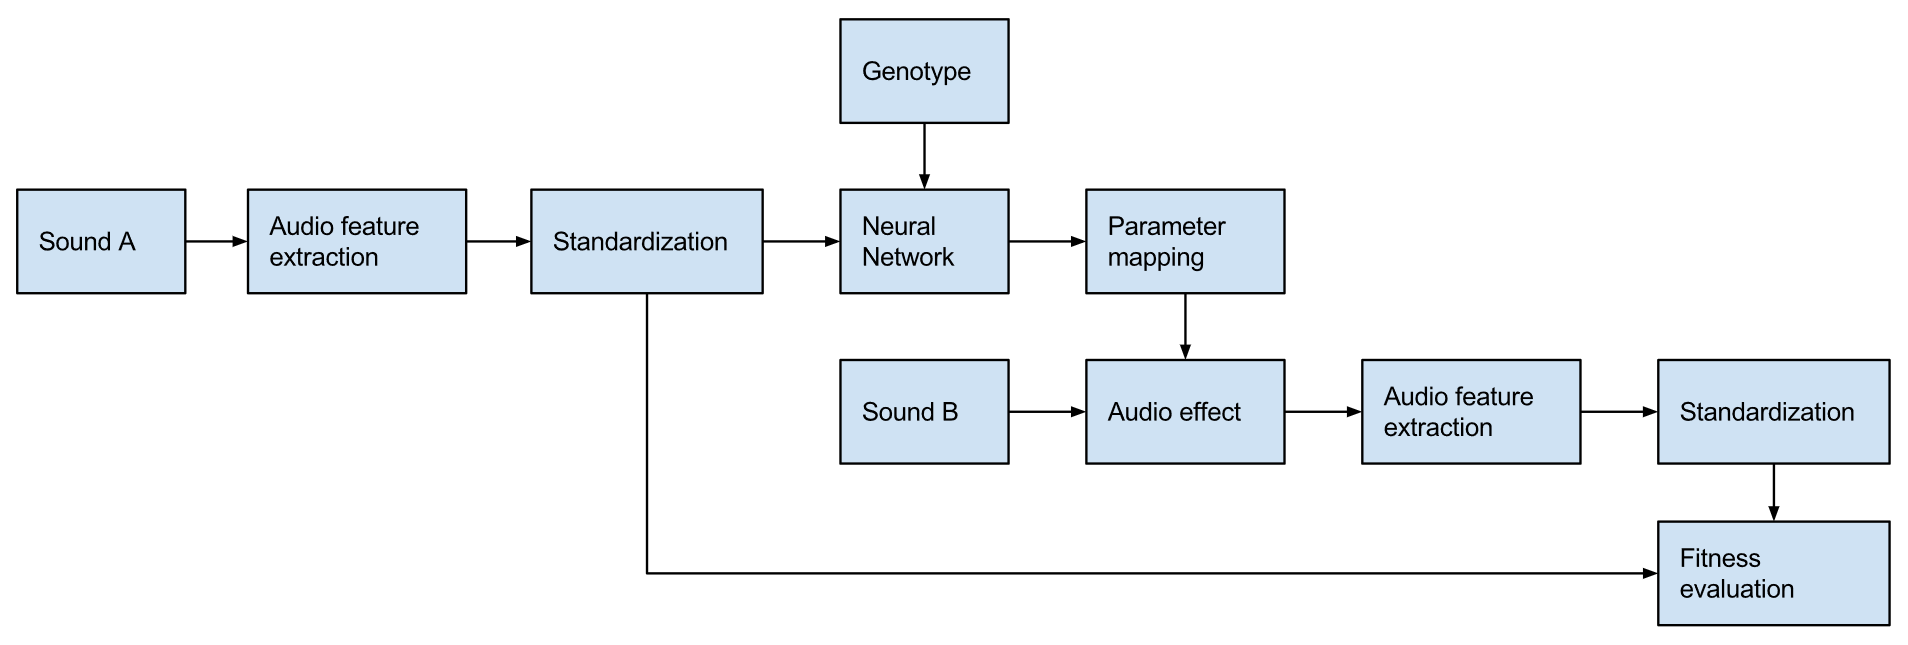
\includegraphics[width=0.99\textwidth]{06_individual_evaluation_process}
    \caption{Flowchart for the evaluation of an individual}
    \label{fig:individual_evaluation_process}
\end{figure}

\subsection{Input standardization}
To make the audio features suitable as input to a neural network, they need to be scaled. A simple, but good technique is to standardize them by is subtracting the mean and dividing by the standard deviation (Sarle, 2014). For each audio feature there is one sequence of numbers for the input sound and another sequence for the target sound. The mean and standard deviation for an audio feature is calculated from the input sound’s sequence for that feature concatenated with the target sound’s sequence for that feature. This mean and standard deviation is then used in all further input standardization. This gives the series the quality of being centered around zero and having a standard deviation of 1 with respect to the input sound and the target sound. Additionally, to avoid extreme values, values are clipped to the range [-4, 4].

\subsection{Parameter mapping}
The output of the neural network is in the range [0, 1], due to the sigmoid activation function in the output layer. These normalized values need to be scaled and skewed appropriately for each effect parameter. The author has used the same mapping function as in Cabbage (Walsh, 2008), a GUI framework for Csound, where slider values are mapped from 0 to 1 to the target range by the following function:

$$f(x)=m_{min}+(m_{max}-m_{min})*e^{\log(x)/s}$$

Where $m_{min}$ and $m_{max}$ are the endpoints of the target range and s is the skew factor. The default skew factor is 1, which will yield a linear mapping. A skew factor of 0.5 will cause the mapping function to output values in an exponential fashion. This is useful for effect parameters such as cutoff frequency.

\section{Visualization}
In very early versions of the neuroevolution program, the author found it hard to evaluate all the data produced during experiments. Therefore an interactive web application for visualizing results was developed. This tool has been very important for being able to understand the strengths and weaknesses of the neuroevolution program during development and research. When the author gained a good understanding of the inner workings and the output of the neuroevolution program, he was able to improve the weak points of the implementation.

The visualization system is a single-page web application written in AngularJS, with various JavaScript libraries for visualizing data. For a complete list of JavaScript libraries that were used in the web application, see appendix C TODO. The application server is written in NodeJS. The neuroevolution program writes data after each generation, and the NodeJS server listens for these data updates. Whenever new data is available, the updated data is sent via WebSockets to the web application, which then updates its views. Figure \ref{fig:viz_fitness_plot}, \ref{fig:viz_species_plot}, \ref{fig:viz_fitness_histogram} and \ref{fig:viz_individual} show partial screenshots the web application.

\begin{figure}[h]
    \centering
    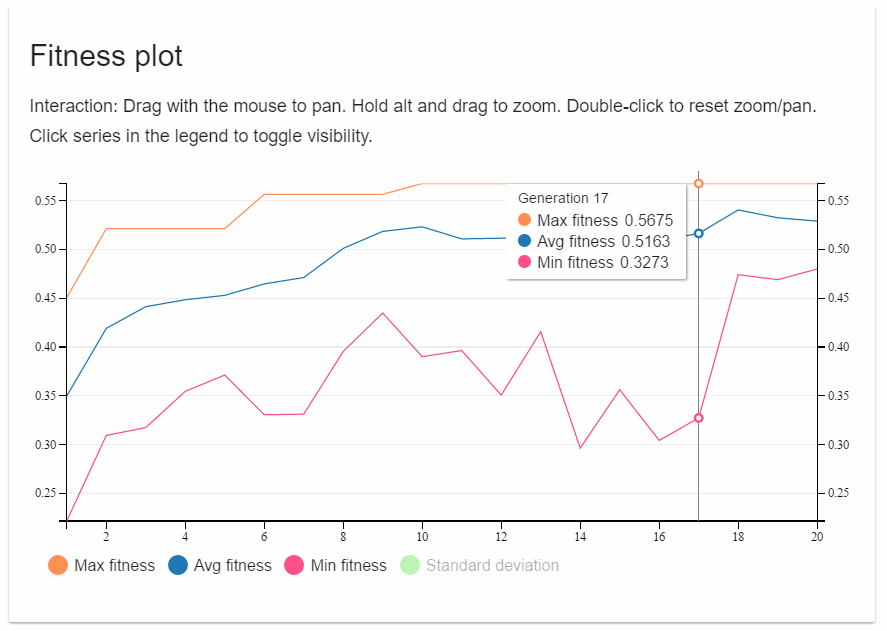
\includegraphics[width=0.99\textwidth]{viz_fitness_plot}
    \caption{Fitness plot (line chart, shows the progress of the GA over the generations)}
    \label{fig:viz_fitness_plot}
\end{figure}

\begin{figure}[h]
    \centering
    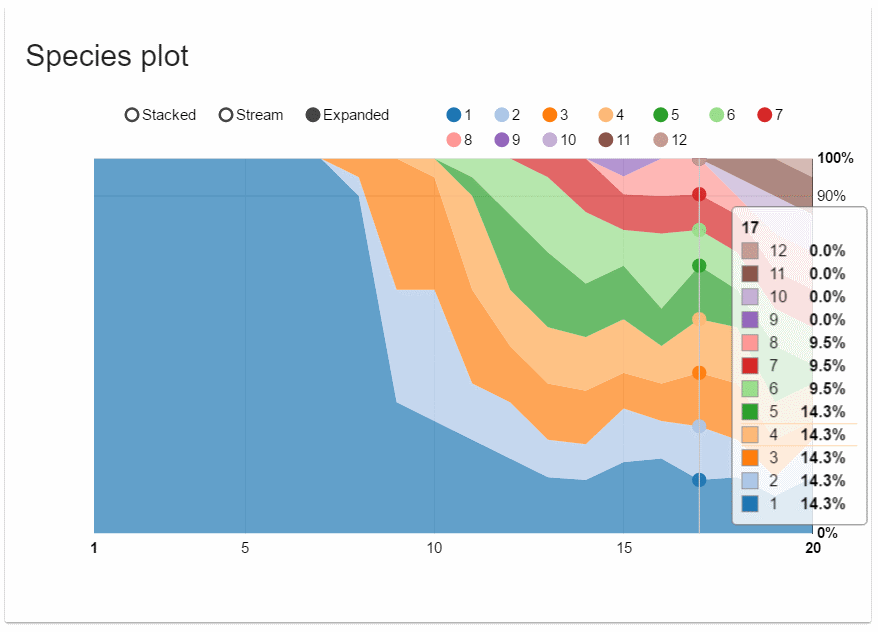
\includegraphics[width=0.99\textwidth]{viz_species_plot}
    \caption{Species plot (stacked area chart, shows the number of individual in each species over the generations)}
    \label{fig:viz_species_plot}
\end{figure}


\begin{figure}[h]
    \centering
    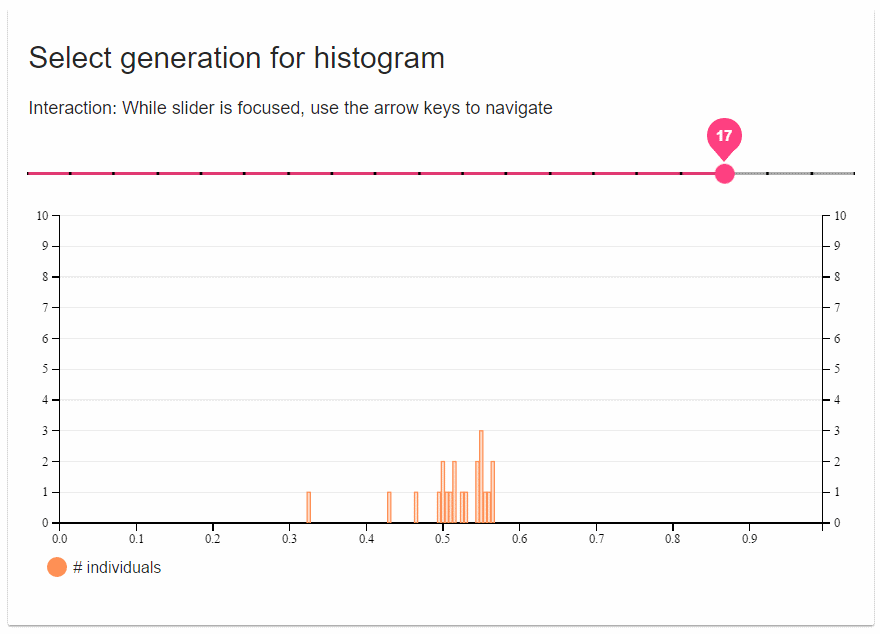
\includegraphics[width=0.99\textwidth]{viz_fitness_histogram}
    \caption{The fitness histogram shows fitness distribution in the population of the generation selected by the interactive slider}
    \label{fig:viz_fitness_histogram}
\end{figure}

\begin{figure}[h]
    \centering
    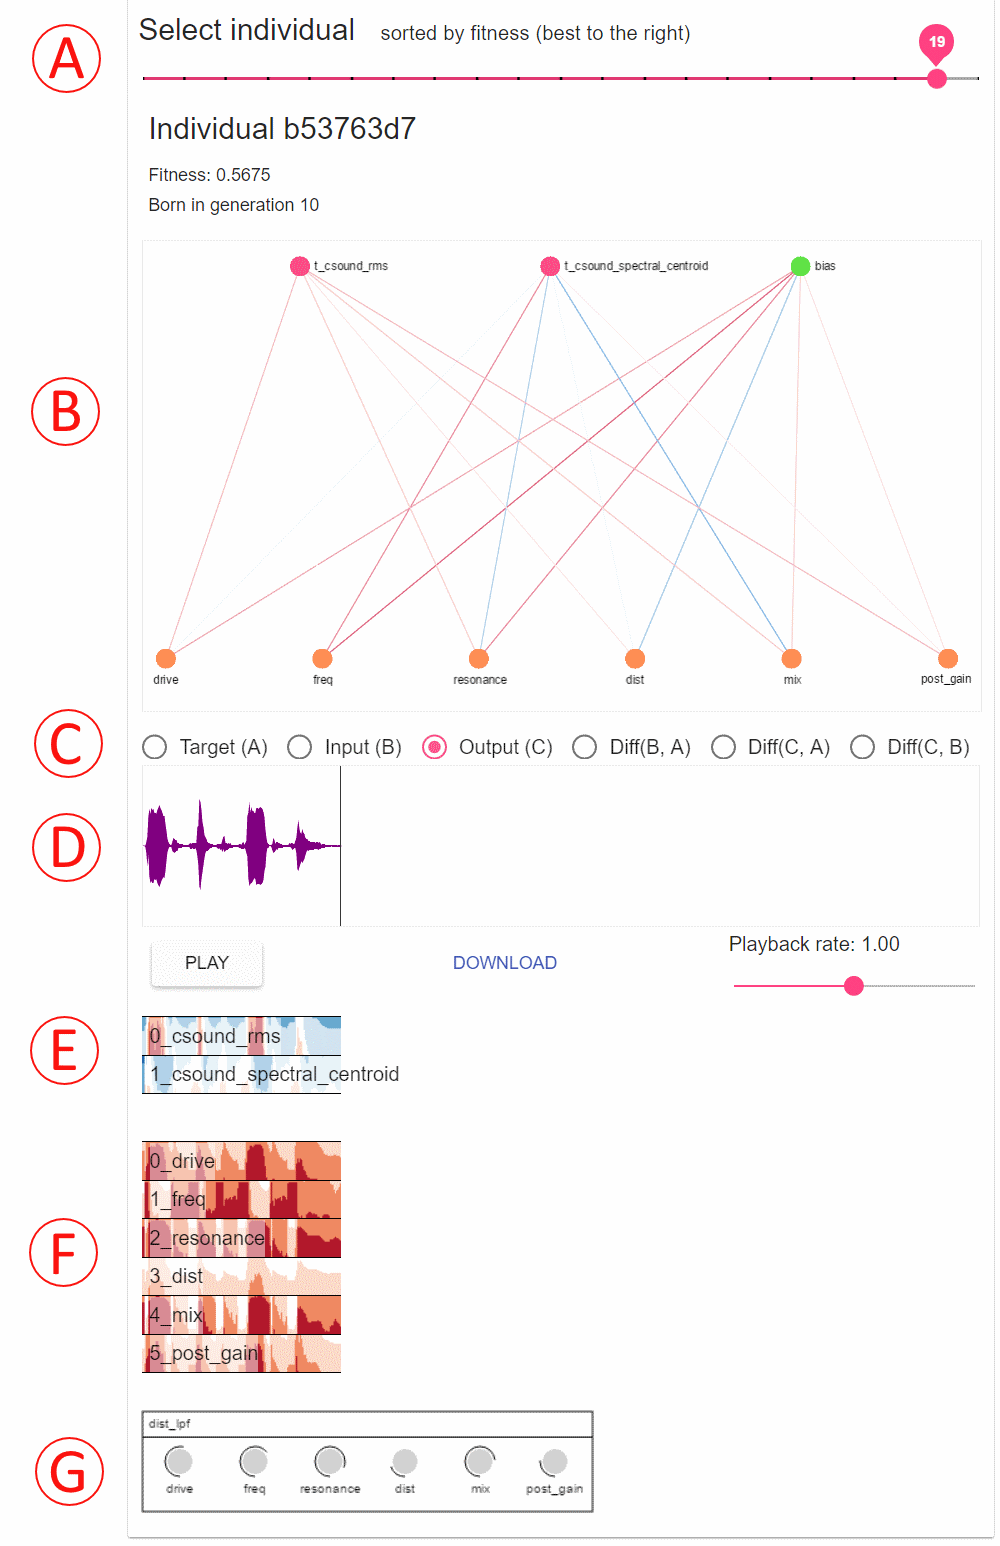
\includegraphics[width=0.65\textwidth]{viz_individual}
    \caption{A: The interactive slider is for selecting a specific individual in the population of the selected generation. B: Neural network visualization with edge colors according to weight. Light color means small magnitude while strong color means large magnitude. Red means positive weight while blue means negative. C: Select which sound and corresponding data series to visualize. D: Audio player with waveform visualization. Useful for playing back the output sound of the selected individual. E and F: Horizon charts for visualizing neural input and neural output, respectively. Horizon charts make better use of vertical space than standard area charts, allowing one to see many more metrics at-a-glance. Larger values are overplotted in successively darker colors, while negative values are offset to descend from the top. When hovering over these charts with the mouse pointer, series labels disappear and a rule with values at the hovered time step is shown. The horizon charts are aligned with the audio player. G: Shows the effect(s) and its parameters. While playing the audio, the knob positions are animated according to the way they were controlled in order to produce the output sound.}
    \label{fig:viz_individual}
\end{figure}



% !TEX encoding = UTF-8 Unicode
%!TEX root = thesis.tex
% !TEX spellcheck = en-US
%%=========================================
\chapter{Experiments and Discussion}
\label{chapter:experiments_and_discussion}

Four experiments have been conducted in an attempt to find good ways to use neuroevolution for finding useful mappings from audio features to audio effect parameters. In each experiment, different neuroevolution configurations are compared to find what works better. Due to the random nature of genetic algorithms, results vary from run to run. To deal with this, each configuration gets multiple runs (with different Pseudo Random Number Generator (PRNG) seeds), and results from the runs are aggregated and presented in various figures. Table \ref{tab:experiments_overview} shows a rough overview of the experiments.

\begin{center}
\begin{longtable}{p{2.3cm} p{13cm}}
\caption[Overview of experiments]{Overview of experiments} \label{tab:experiments_overview} \\

\hline \multicolumn{1}{l}{\textbf{Experiment}} & \multicolumn{1}{l}{\textbf{Description}} \\ \hline 
\endfirsthead

\multicolumn{2}{c}%
{{\bfseries \tablename\ \thetable{} -- continued from previous page}} \\
\hline \multicolumn{1}{l}{\textbf{Experiment}} & \multicolumn{1}{l}{\textbf{Description}} \\ \hline 
\endhead

\hline \multicolumn{2}{r}{{Continued on next page}} \\ \hline
\endfoot

\hline \hline
\endlastfoot

\midrule
  1 & Find the best combination of mutation rate and crossover rate \\
\midrule
  2 & Find a good value for structural mutation parameters \\
\midrule
  3 & Compare sets of audio features used in the fitness function. Analyze data from the neuroevolution process. \\
\midrule
  4 & Compare networks of audio effects with individual audio effects. \\
\end{longtable}
\end{center}

\section{General Configuration}
Table \ref{tab:general_configuration} shows the parameters used unless otherwise stated in individual experiments

\begin{center}
\begin{longtable}{p{10cm} p{4cm}}
\caption[General experiment configuration]{General experiment configuration} \label{tab:general_configuration} \\

\hline \multicolumn{1}{l}{\textbf{Parameter}} & \multicolumn{1}{l}{\textbf{Value}} \\ \hline 
\endfirsthead

\multicolumn{2}{c}%
{{\bfseries \tablename\ \thetable{} -- continued from previous page}} \\
\hline \multicolumn{1}{l}{\textbf{Parameter}} & \multicolumn{1}{l}{\textbf{Value}} \\ \hline 
\endhead

\hline \multicolumn{2}{r}{{Continued on next page}} \\ \hline
\endfoot

\hline \hline
\endlastfoot

\midrule
  Population size & 20 \\
\midrule
  Add neuron probability & 0.01 \\
\midrule
  Remove neuron probability & 0.01 \\
\midrule
  Add link probability & 0.01 \\
\midrule
  Remove link probability & 0.01 \\
\midrule
  Elite fraction & 0.1 \\
\midrule
  Survival rate & 0.25 \\
\midrule
  Allow clones & Yes \\
\midrule
  Selection method & Tournament selection \\
\midrule
  Hidden activation function & Hyperbolic tangent \\
\midrule
  Output activation function & Sigmoid \\
\midrule
  Effect parameter low-pass filter cutoff frequency & 50 Hz \\
\midrule
  Fitness function & Local similarity \\
\end{longtable}
\end{center}

% !TEX encoding = UTF-8 Unicode
%!TEX root = thesis.tex
% !TEX spellcheck = en-US
%%=========================================
\section{Experiment 1}
In this experiment, the aim is to find good values for crossover rate and mutation rate.

\subsection{Configuration}

\begin{center}
\begin{longtable}{p{5cm} p{7cm}}
\caption[Experiment configuration]{Experiment configuration} \label{tab:exp1_configuration} \\

\hline \multicolumn{1}{l}{\textbf{Parameter}} & \multicolumn{1}{l}{\textbf{Value}} \\ \hline 
\endfirsthead

\multicolumn{2}{c}%
{{\bfseries \tablename\ \thetable{} -- continued from previous page}} \\
\hline \multicolumn{1}{l}{\textbf{Parameter}} & \multicolumn{1}{l}{\textbf{Value}} \\ \hline 
\endhead

\hline \multicolumn{2}{r}{{Continued on next page}} \\ \hline
\endfoot

\hline \hline
\endlastfoot

Number of generations & 20 \\
\midrule
Target sound & Drum loop \\
\midrule
Input sound & White noise \\
\midrule
Effect & Distortion and resonant low-pass filter \\
\midrule
Audio features & mfcc\_0, mfcc\_0\_\_derivative, mfcc\_1 \\
\midrule
Number of runs & 150 per configuration \\
\end{longtable}
\end{center}

\subsection{Results and evaluation}
Figure \ref{fig:exp1_heatmap} shows that one should avoid using a high mutation rate and a low crossover rate. Instead, one of the combinations inside the red region should do well. Bear in mind that the differences between pure yellow and lime green are small in this region, and that these small differences are not statistically significant. The variance could be reduced with more runs, but due to computational time, the number of runs per configuration was limited to 150. The yellow spot is probably a good configuration, albeit not necessarily the best. Muration rate = 0.6 and crossover rate = 0.7 are used in the following experiments.

\begin{figure}[H]
    \centering
    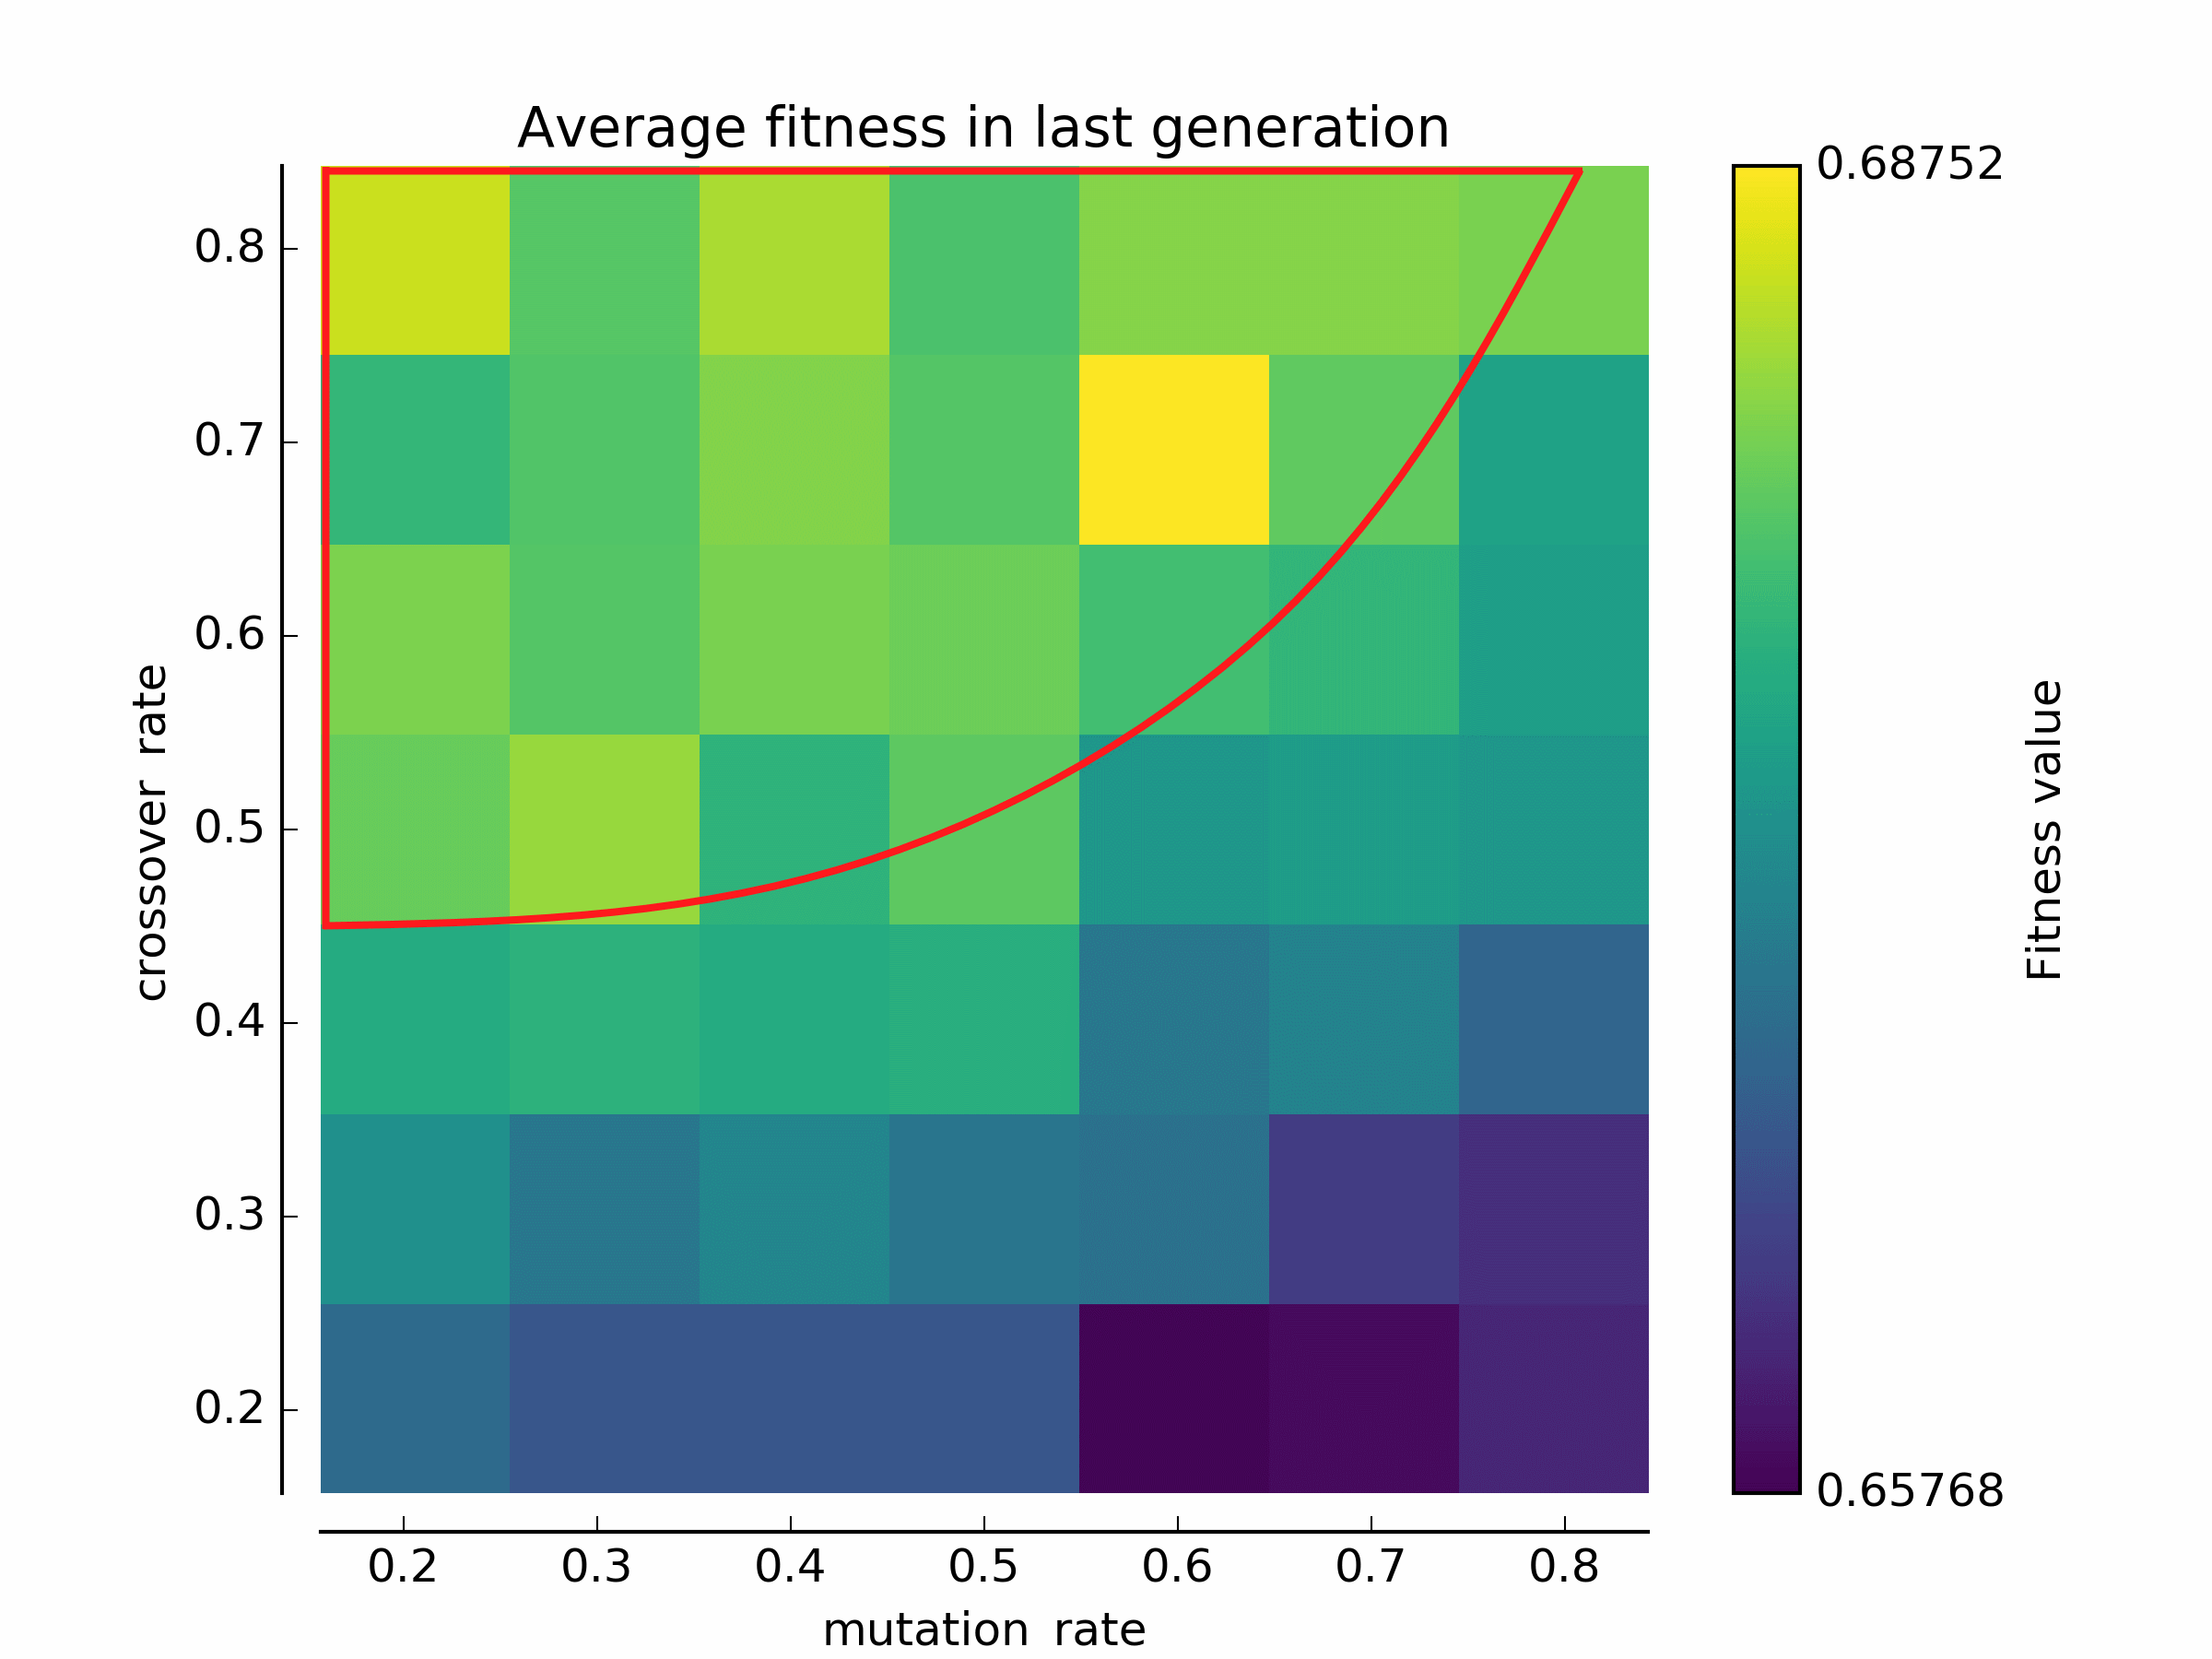
\includegraphics[width=0.99\textwidth]{grid_search_crossover_mutation_avg}
    \caption{The red region drawn on top of the heat map indicates the set of configurations deemed good}
    \label{fig:exp1_heatmap}
\end{figure}
% !TEX encoding = UTF-8 Unicode
%!TEX root = thesis.tex
% !TEX spellcheck = en-US
%%=========================================
\section{Experiment 2}
In this experiment, the aim is to find a good value for add link probability et al TODO

\subsection{Configuration}
\begin{minipage}{\linewidth}
\centering
\captionof{table}{Table Title TODO} \label{tab:title} 
\begin{tabular}{ C{3.5in} C{1.6in} }\toprule[1.5pt]
\bf Parameter & \bf Value \\
\midrule
  Number of generations & 50 \\
\midrule
  Fitness function & Local similarity \\
\midrule
  Target sound & Drum loop \\
\midrule
  Input sound & White noise \\
\midrule
  Effect & Distortion and resonant low-pass filter \\
\midrule
  Audio features & mfcc\_0, mfcc\_0\_\_derivative, mfcc\_1 \\
\midrule
  Number of runs & 400 per configuration \\
\bottomrule[1.25pt]
\end {tabular}\par
\bigskip
Should be a caption TODO
\end{minipage}

\subsection{Fitness function}
Same as in experiment 1

\subsection{Evaluation of configurations}
Figure \ref{fig:add_link_probability} TODO shows that 0.03 is probably the best value while 0.3 is significantly worse

\begin{figure}[h]
    \centering
    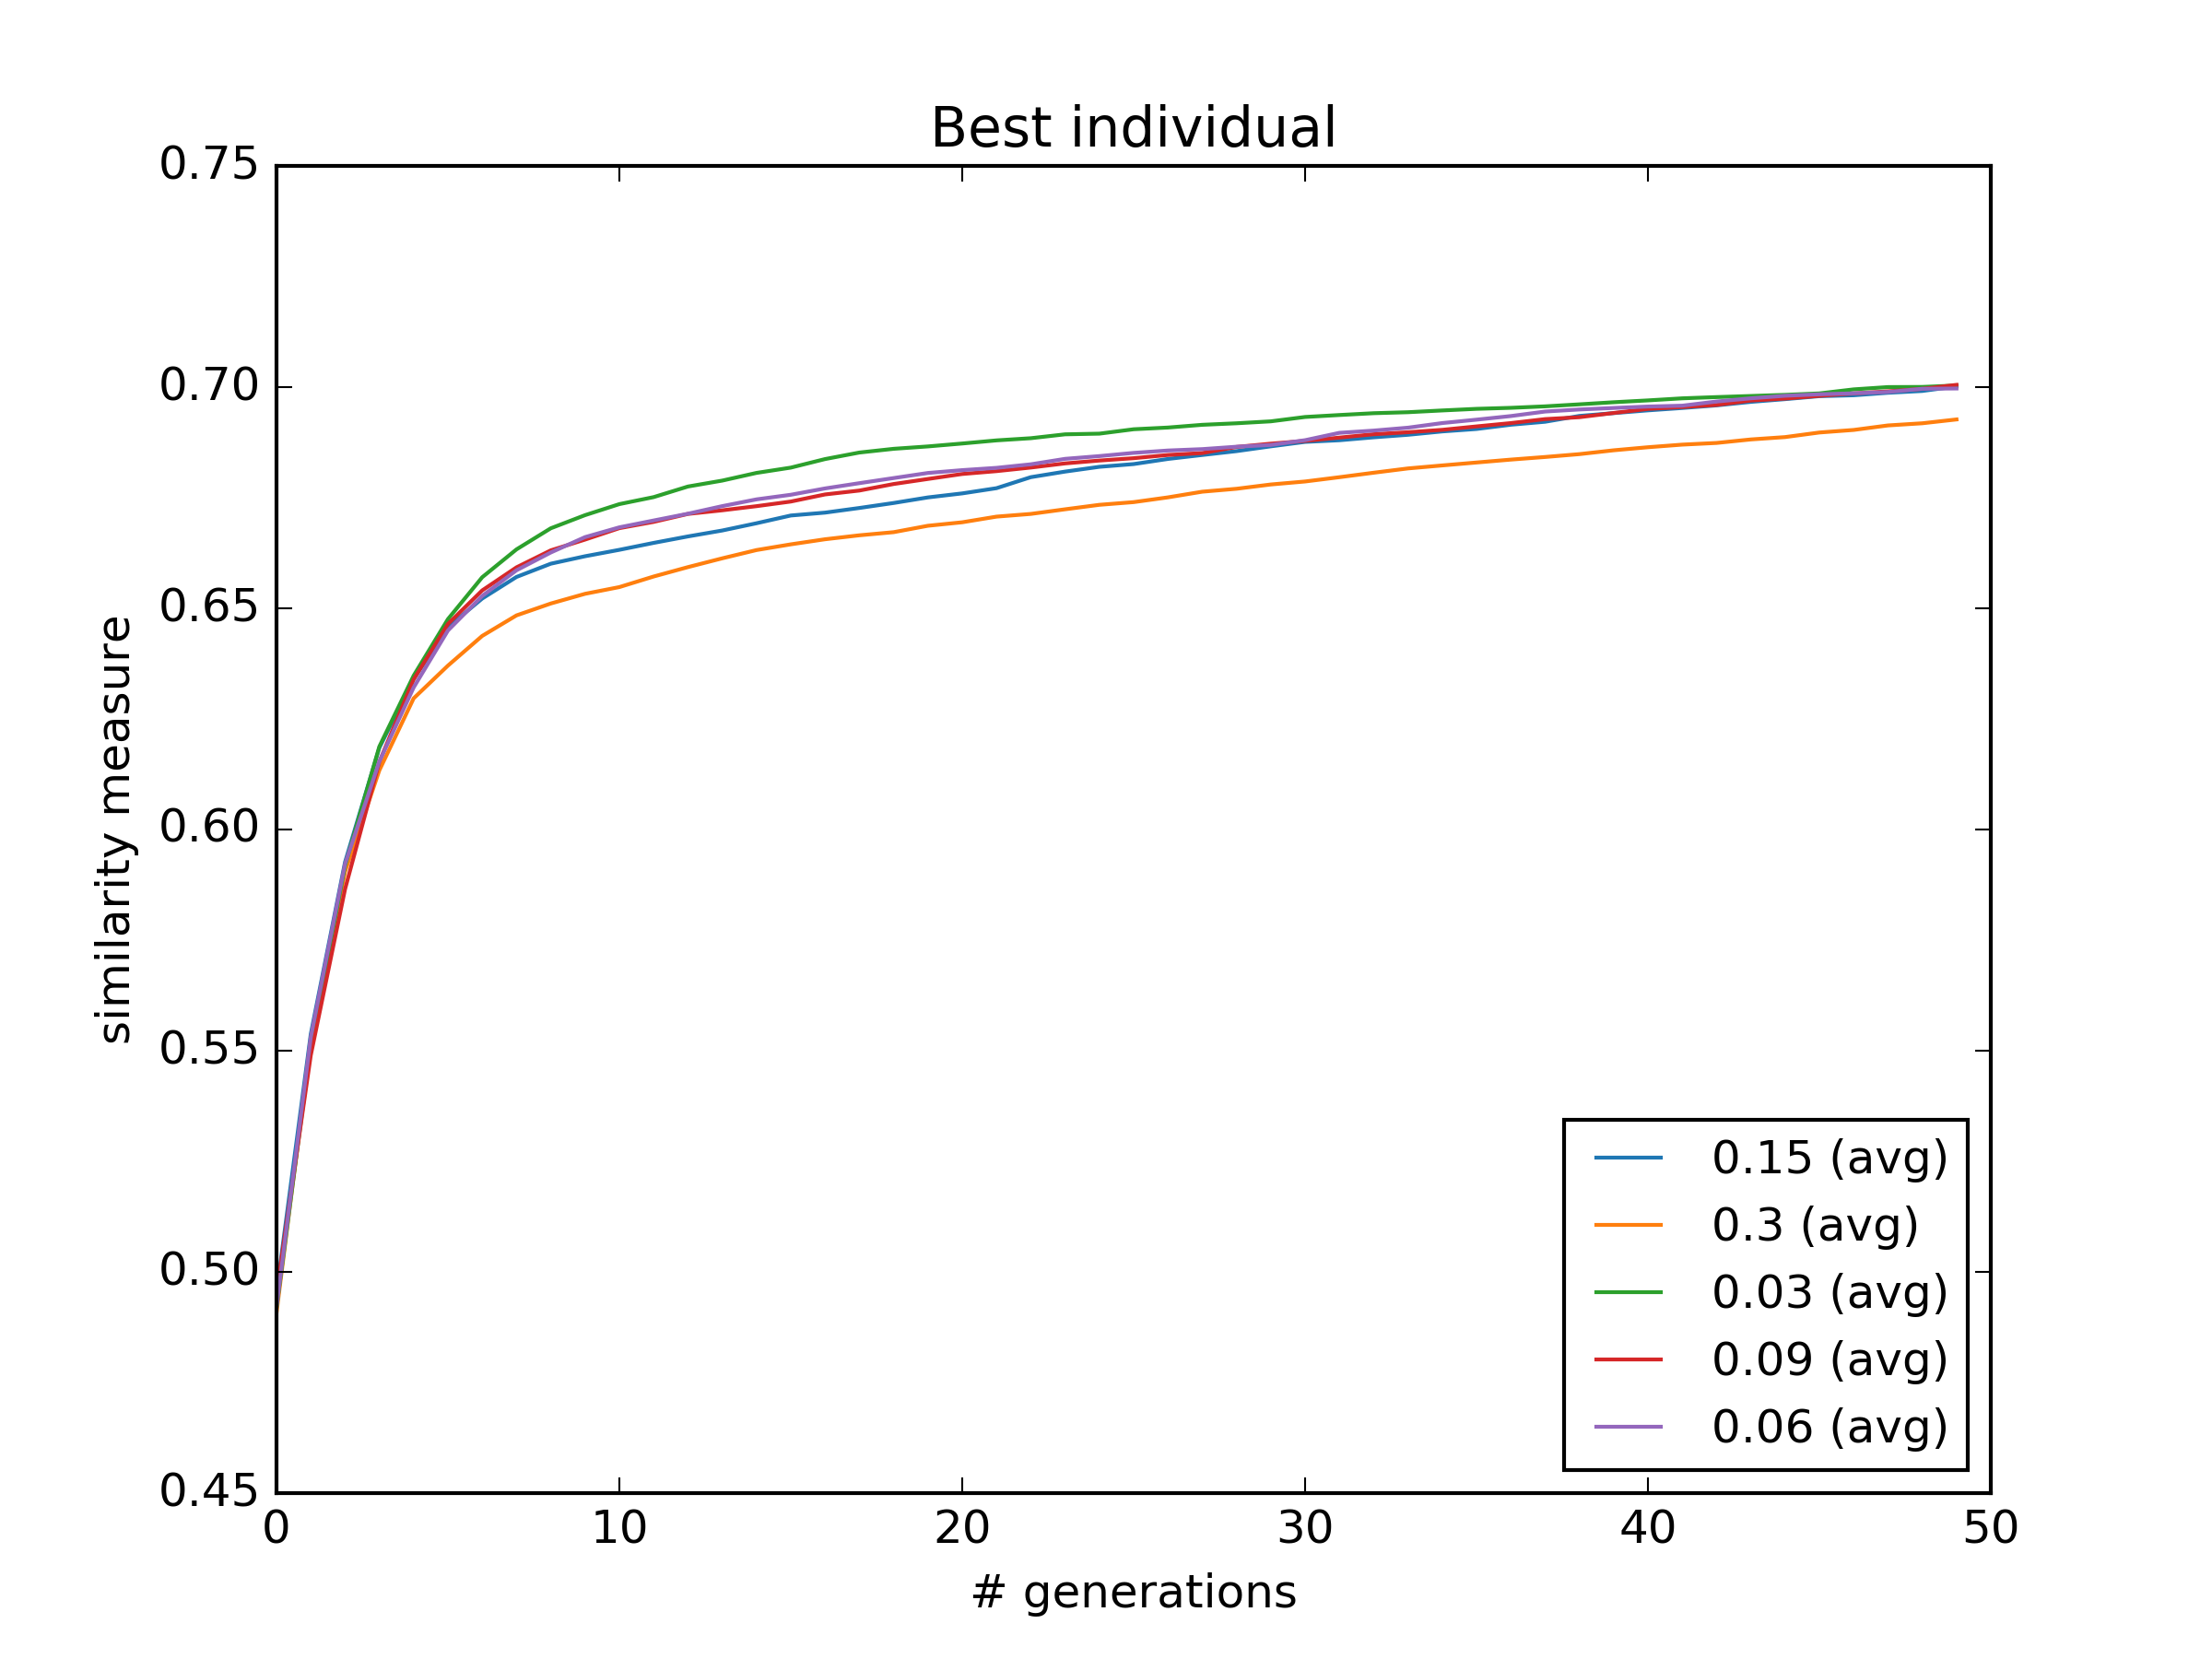
\includegraphics[width=0.99\textwidth]{add_link_probability}
    \caption{TODO caption}
    \label{fig:add_link_probability}
\end{figure}

TODO: Show typical end-result neural networks from all the configurations, to highlight that higher probability builds a larger, more complex network

% !TEX encoding = UTF-8 Unicode
%!TEX root = thesis.tex
% !TEX spellcheck = en-US
%%=========================================
\section{Experiment 3}
When using an evolved cross-adaptive audio effect in a live performance, a performer may want to use it in an expressive way. For example, if the performer is a drummer, he can vary the intensity of the drum hits. For the cross-adaptive audio effect to handle this, it needs to be trained on all the different intensities of the drum hits. If an extensive recording is available, that is fine. However, if the available target sound is short or lacks sufficient variation, one can harness the concept of data augmentation to create artificial variations of that sound. If one uses that sound instead, the evolved effect will typically be more capable of dealing with the generated variations. This experiment is about testing the author's implementation of data augmentation and the ability to apply evolved cross-adaptive audio effects to unseen sounds.

% TODO: mention the sounds and how augmented

\subsection{Configuration}

\begin{center}
\begin{longtable}{p{5cm} p{7cm}}
\caption[Experiment configuration]{Experiment configuration} \label{tab:exp3_configuration} \\

\hline \multicolumn{1}{l}{\textbf{Parameter}} & \multicolumn{1}{l}{\textbf{Value}} \\ \hline 
\endfirsthead

\multicolumn{2}{c}%
{{\bfseries \tablename\ \thetable{} -- continued from previous page}} \\
\hline \multicolumn{1}{l}{\textbf{Parameter}} & \multicolumn{1}{l}{\textbf{Value}} \\ \hline 
\endhead

\hline \multicolumn{2}{r}{{Continued on next page}} \\ \hline
\endfoot

\hline \hline
\endlastfoot

Number of generations & 20 \\
\midrule
Target sound (training) & Drum loop with bass drum, snare drum, clap and hihat (figure \ref{fig:exp3_waveforms}) \\
\midrule
Target sound (validation) & Snare roll (rapid snare drum hits) with ascending pitch and amplitude (figure \ref{fig:exp3_waveforms}) \\
\midrule
Input sound & White noise \\
\midrule
Effect & Distortion and resonant low-pass filter \\
\midrule
Audio features & Root Mean Square (RMS) and spectral centroid \\
\midrule
Number of runs & 40 per configuration \\
\end{longtable}
\end{center}

\begin{figure}[H]
    \centering
    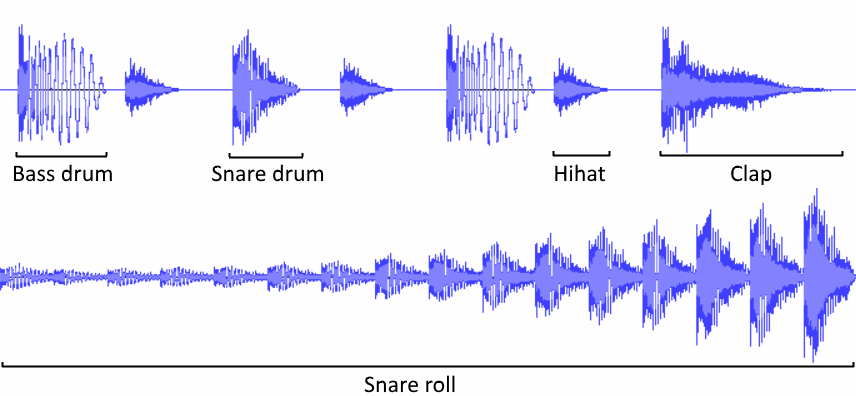
\includegraphics[width=1.0\textwidth]{exp3_waveforms}
    \caption{Waveform of training sound (top) and validation sound (bottom)}
    \label{fig:exp3_waveforms}
\end{figure}

The augmented variant of the training sound was created by repeating the sound 8 times, with variations in playback speed and gain for each repetition. The playback speed and gain are sampled from a gaussian distribution centered around $1$ and with standard deviations of $0.3$ and $0.5$, respectively.

%TODO: mention exponential thingy


\subsection{Results and evaluation}
Figure \ref{fig:exp3_fitness_box} shows that neural networks trained on an augmented variant of the training sound generalizes better than the raw training sound.

% Helps in live settings which typically play in more nuanced ways than the sounds the network is pre-trained on

\begin{figure}[H]
    \centering
    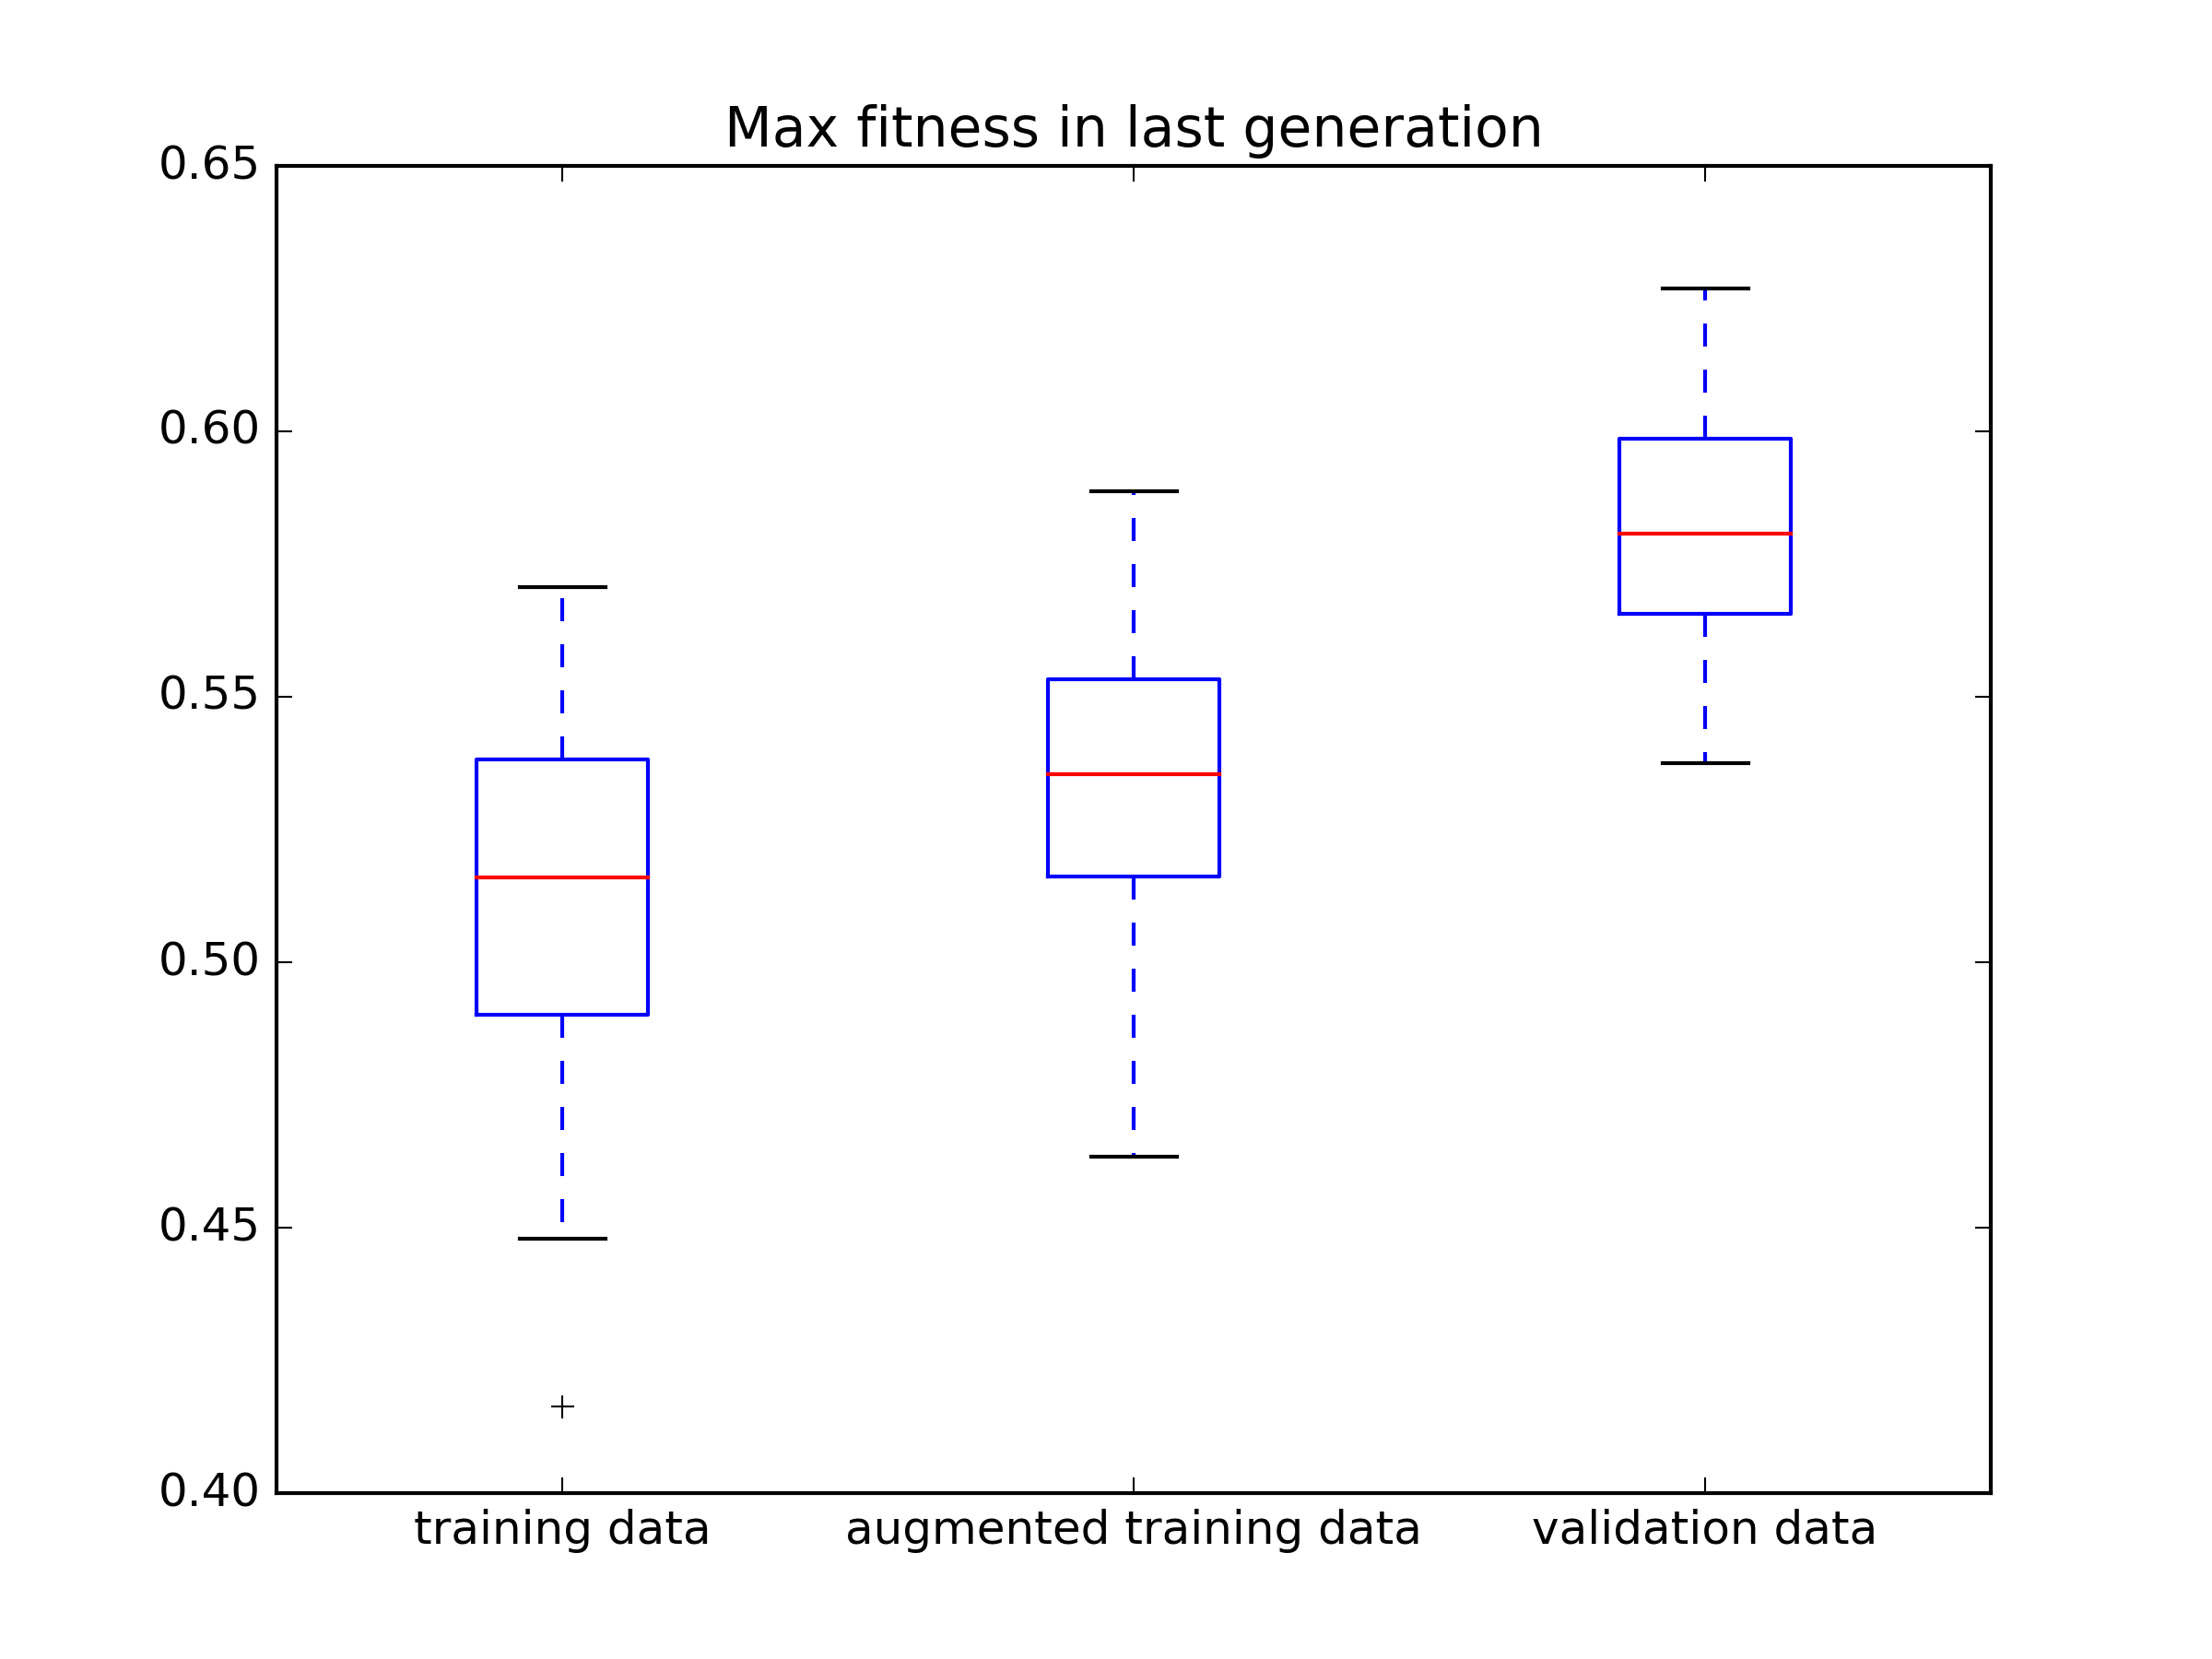
\includegraphics[width=1.0\textwidth]{exp3_fitness_box}
    \caption{Box plot of validation fitness values in final generation. The labels on the x-axis indicate which sound was used as target sound.}
    \label{fig:exp3_fitness_box}
\end{figure}

% !TEX encoding = UTF-8 Unicode
%!TEX root = thesis.tex
% !TEX spellcheck = en-US
%%=========================================
\section{Experiment 3} % TODO: Rename to Experiment 4 if I ever finish and include Experiment 3

\subsection{Configuration}
In this experiment, the aim is to compare two different collections of audio features used in the similarity measure:

\begin{itemize}
\item Configuration A: RMS, pitch and spectral centroid
\item Configuration B: RMS, pitch, spectral centroid and bark bands
\end{itemize}

\begin{center}
\begin{longtable}{p{5cm} p{7cm}}
\caption[Experiment configuration]{Experiment configuration} \label{tab:exp4_configuration} \\

\hline \multicolumn{1}{l}{\textbf{Parameter}} & \multicolumn{1}{l}{\textbf{Value}} \\ \hline 
\endfirsthead

\multicolumn{2}{c}%
{{\bfseries \tablename\ \thetable{} -- continued from previous page}} \\
\hline \multicolumn{1}{l}{\textbf{Parameter}} & \multicolumn{1}{l}{\textbf{Value}} \\ \hline 
\endhead

\hline \multicolumn{2}{r}{{Continued on next page}} \\ \hline
\endfoot

\hline \hline
\endlastfoot

\midrule
Number of generations & 500 \\
\midrule
Target sound & Sine wave, 440 Hz \\
\midrule
Input sound & White noise \\
\midrule
Effect & Band-pass filter with up to 10x post gain \\
\midrule
Number of runs & 20 per configuration \\
\end{longtable}
\end{center}

\subsection{Results and evaluation}
Since fitness functions were different in these two configurations, the fitness values are not directly comparable. Instead, the results were evaluated by manually listening to the output sounds. In the first configuration, the results were fairly bad: All of the sounds were too noisy, and the author failed to perceive the tone. However, in terms of spectral centroid and amplitude, the sounds were a good match. In order to transform noise into a sine, the bandwidth of the band-pass filter has to be very narrow. A narrow filter would have lowered the overall amplitude of the sound. This would have been deemed bad by the fitness function, hence the genetic algorithm did not effectively explore that area in the solution space. Also, a narrow filter would not have yielded any improvements in the similarity in spectral centroid and/or pitch. Therefore, the typical solution has a broad bandpass filter, albeit with an appropriate center frequency. See in figure \ref{fig:exp4_spectrum_plot} that the peak frequency of the typical output sound matches well the peak frequency of the target sound.

The results in the second configuration, were much better. The author could hear a clear tone in all 10 output sounds. There was still some noise in most sounds. The author believes that the solutions would have improved with more generations, because the fitness was typically still increasing towards the 500th (last) generation. One of the output sounds featured vibrato (varying pitch over time), due to a noisy input being mapped to the center frequency parameter. This could probably have been alleviated by adding the derivative of the pitch as a dimension in the fitness function, so the unwanted vibrato would be punished more severely by the fitness function.

\begin{figure}[h]
    \centering
    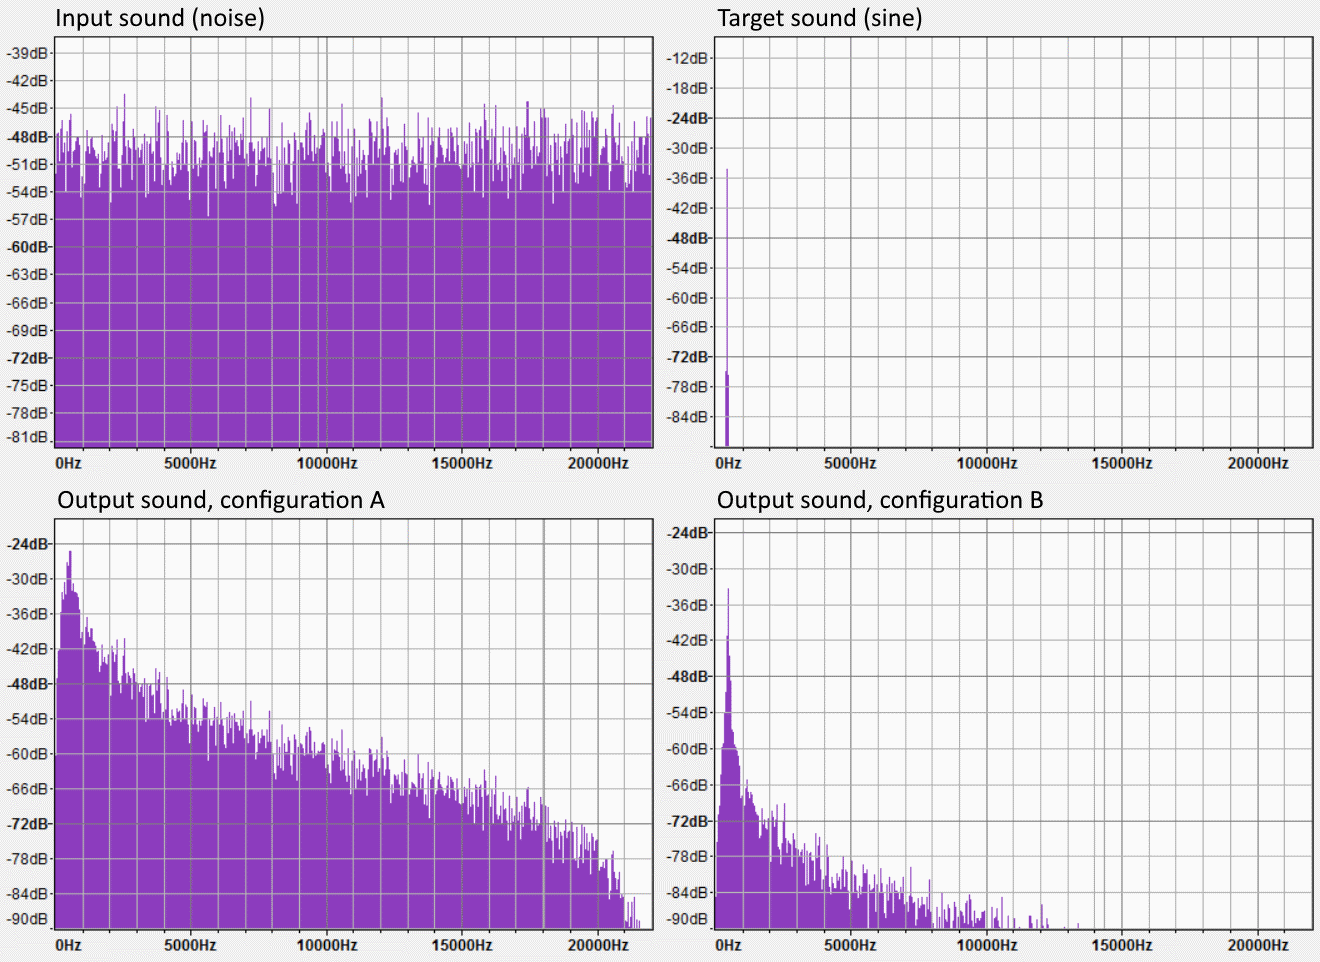
\includegraphics[width=1.0\textwidth]{exp4_spectrum_plot}
    \caption{Spectrum plots, created in Audacity® with hanning window of size 8192}
    \label{fig:exp4_spectrum_plot}
\end{figure}

The takeaway from this experiment is that
\begin{itemize}  
\item the collection of features used for similarity measures has a high impact on the result
\item bark bands are useful
\end{itemize}

\subsection{Neuroevolution analysis}

In this subsection, one of the runs in configuration B will be analyzed, to get a better understanding of how NEAT works in practice, and identify some things that can be improved upon.

In this experiment, the effect parameters do not have to be \textit{dynamically} controlled over time. A static value for each effect parameter (bandwidth, center frequency and post gain) would have been an optimal solution. However, in figure \ref{fig:exp4_typical_nn_evolution}, we see that the NEAT algorithm actually makes use all three input nodes (RMS, pitch and spectral centroid) as well as the constand bias node. The reason for this is that these three inputs do not vary much in the course of the sound, because the features of the sound that was analyzed (sine, 440 Hz) do not vary much over time (see figure \ref{fig:exp4_neural_input}). Consequently, these three nodes act like a bias node with some noise.

\begin{figure}[H]
    \centering
    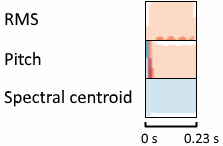
\includegraphics[width=0.3\textwidth]{exp4_neural_input}
    \caption{Neural inputs are almost constant}
    \label{fig:exp4_neural_input}
\end{figure}

\begin{figure}[H]
    \centering
    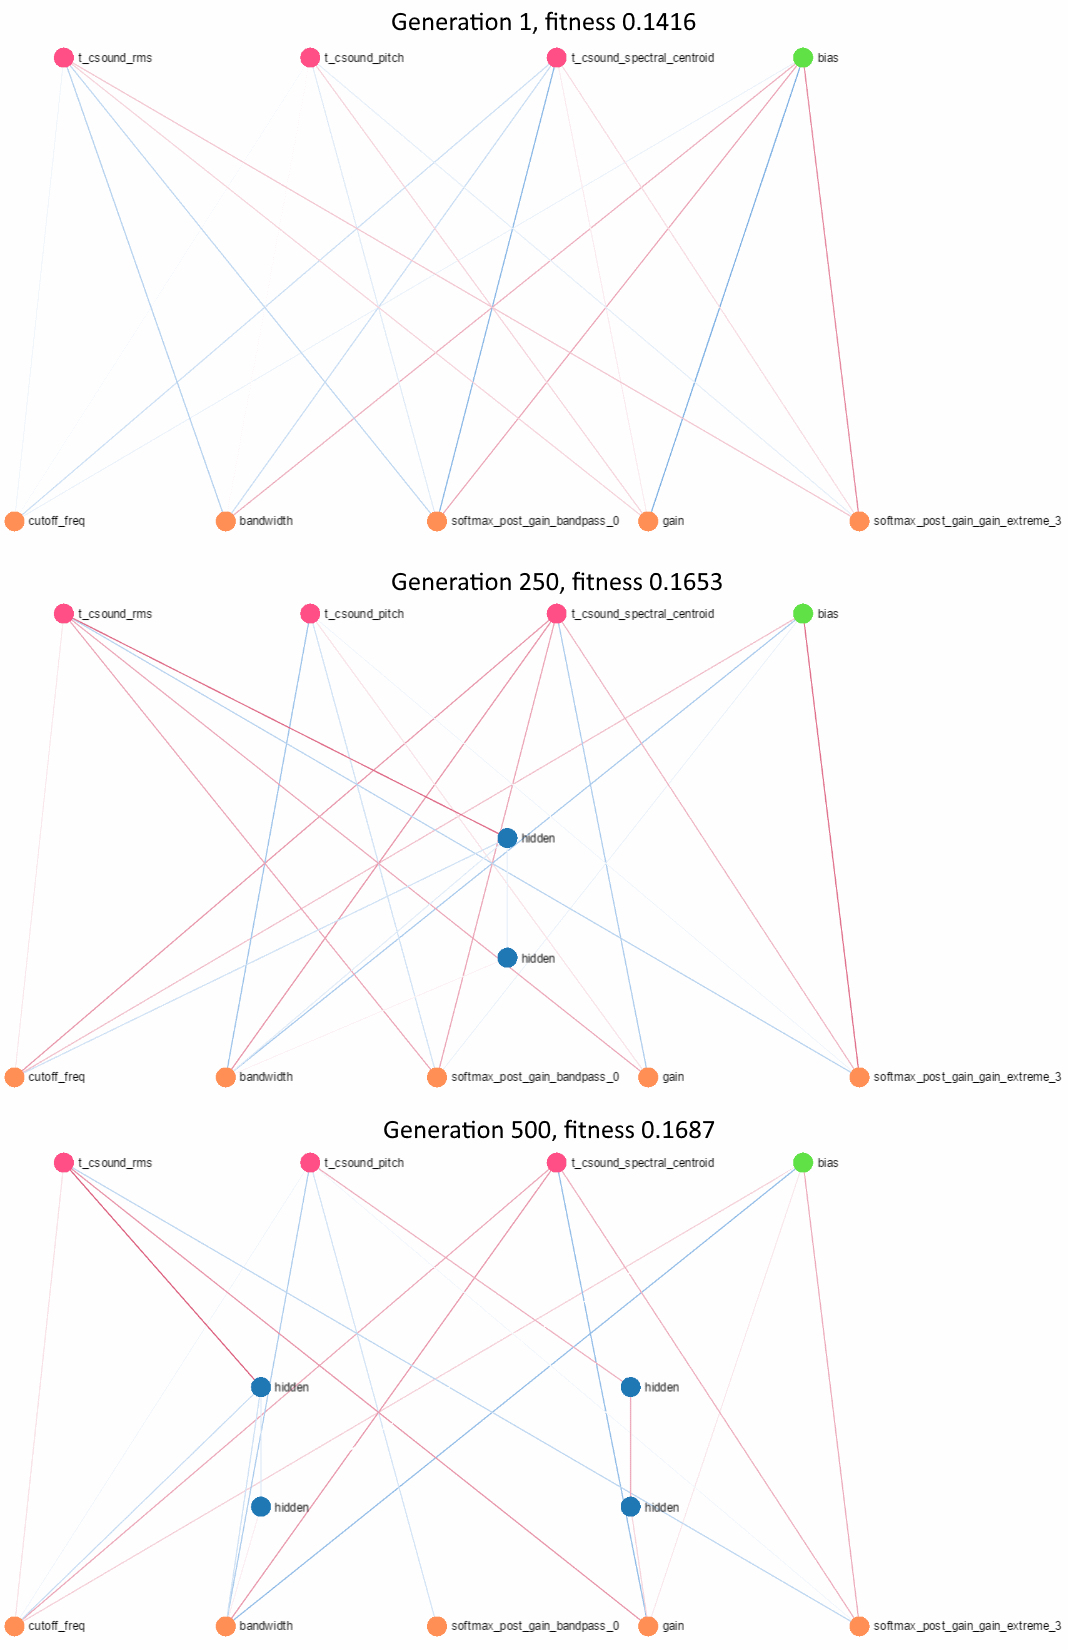
\includegraphics[width=0.9\textwidth]{exp4_typical_nn_evolution}
    \caption{Neural network visualizations}
    \label{fig:exp4_typical_nn_evolution}
\end{figure}

Another interesting fact is that the number of hidden nodes in the best individual tends to increase over the generations, even though these hidden nodes are not needed to get an optimal solution in this experiment. Any constant value can be sent to the output node without having to go through hidden nodes. This is another example of NEAT not finding the optimal solution. Having many hidden nodes hurts evolvability, because an arbitrary mutation on a complex individual is less likely to yield an improvement than the same operation on a simpler individual with fewer hidden nodes. Some form of regularization (punishment for more complex neural networks) could alleviate the problem. Another way to deal with this problem in experiments that do not require hidden nodes is setting AddNodeProbability to zero.

\begin{figure}[H]
    \centering
    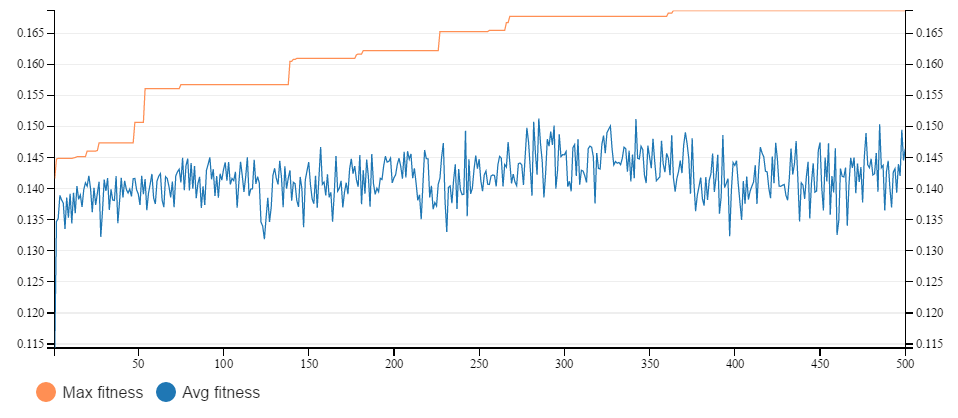
\includegraphics[width=1.0\textwidth]{exp4_fitness_plot}
    \caption{Fitness plot}
    \label{fig:exp4_fitness_plot}
\end{figure}

\begin{figure}[H]
    \centering
    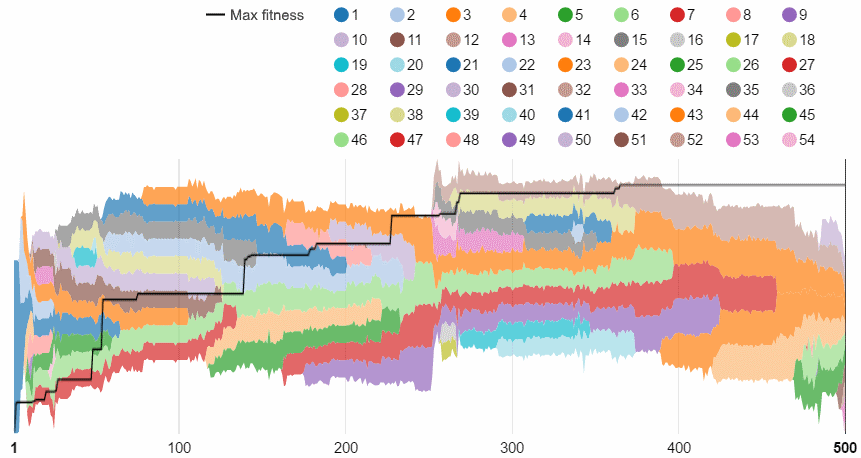
\includegraphics[width=1.0\textwidth]{exp4_species_plot}
    \caption{Species chart with max fitness overlay}
    \label{fig:exp4_species_plot}
\end{figure}

A total of 54 different species were created during the 500 generations of neuroevolution (see figure \ref{fig:exp4_species_plot}). There is no obvious correlation between jumps in max fitness and the death of existing species or the emergence of new species. This makes sense, as competition happens only within species, and species are given time to improve their structure before competition with the rest of the population occurs. The figure also illustrates that the number of species in any given generation is well regulated. The concept of dynamic compatibility threshold in NEAT strives to ensure that the number of species stays within bounds \citep{stanley2004}.

% !TEX encoding = UTF-8 Unicode
%!TEX root = thesis.tex
% !TEX spellcheck = en-US
%%=========================================
\section{Experiment 5}
This experiment is about combining several effects in serial and parallel. The hypothesis is that a genetic algorithm could be adept at choosing which effects to use and how.

For baseline performance measure, each effect has been tested separately. Then they were run in parallel TODO



In this experiment, we do 5 fx in parallel => ok result
am
bandpass
bitreduce
dist lpf
chorus

(Then 2 layers of 5?)
Then 10 fx in parallel => bad result

Suggest pre-training with each fx separately, then training the mix
Softmax mixing may also be bad -> suggest independent mix values

create video demonstrating 1st successful result here

Say something about hypothesis about which fx will be used. Which ones were actually used? Do the same for parameters. Show mix values in horizon graph. Say that am and chorus make sound richer, while we need it filtered.

\begin{figure}[h]
    \centering
    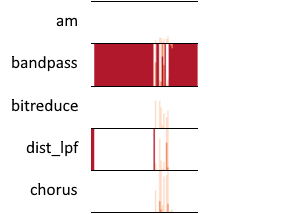
\includegraphics[width=0.45\textwidth]{exp5_1layer_softmax}
    \caption{Gain values for each effect in the best result with configuration 1 TODO}
    \label{fig:exp5_1layer_softmax}
\end{figure}

\begin{figure}[h]
    \centering
    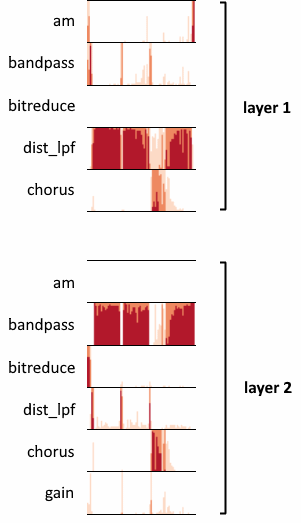
\includegraphics[width=0.45\textwidth]{exp5_2layers_softmax}
    \caption{Gain values for each effect in the best result with configuration 2 TODO}
    \label{fig:exp5_2layers_softmax}
\end{figure}

\begin{figure}[h]
    \centering
    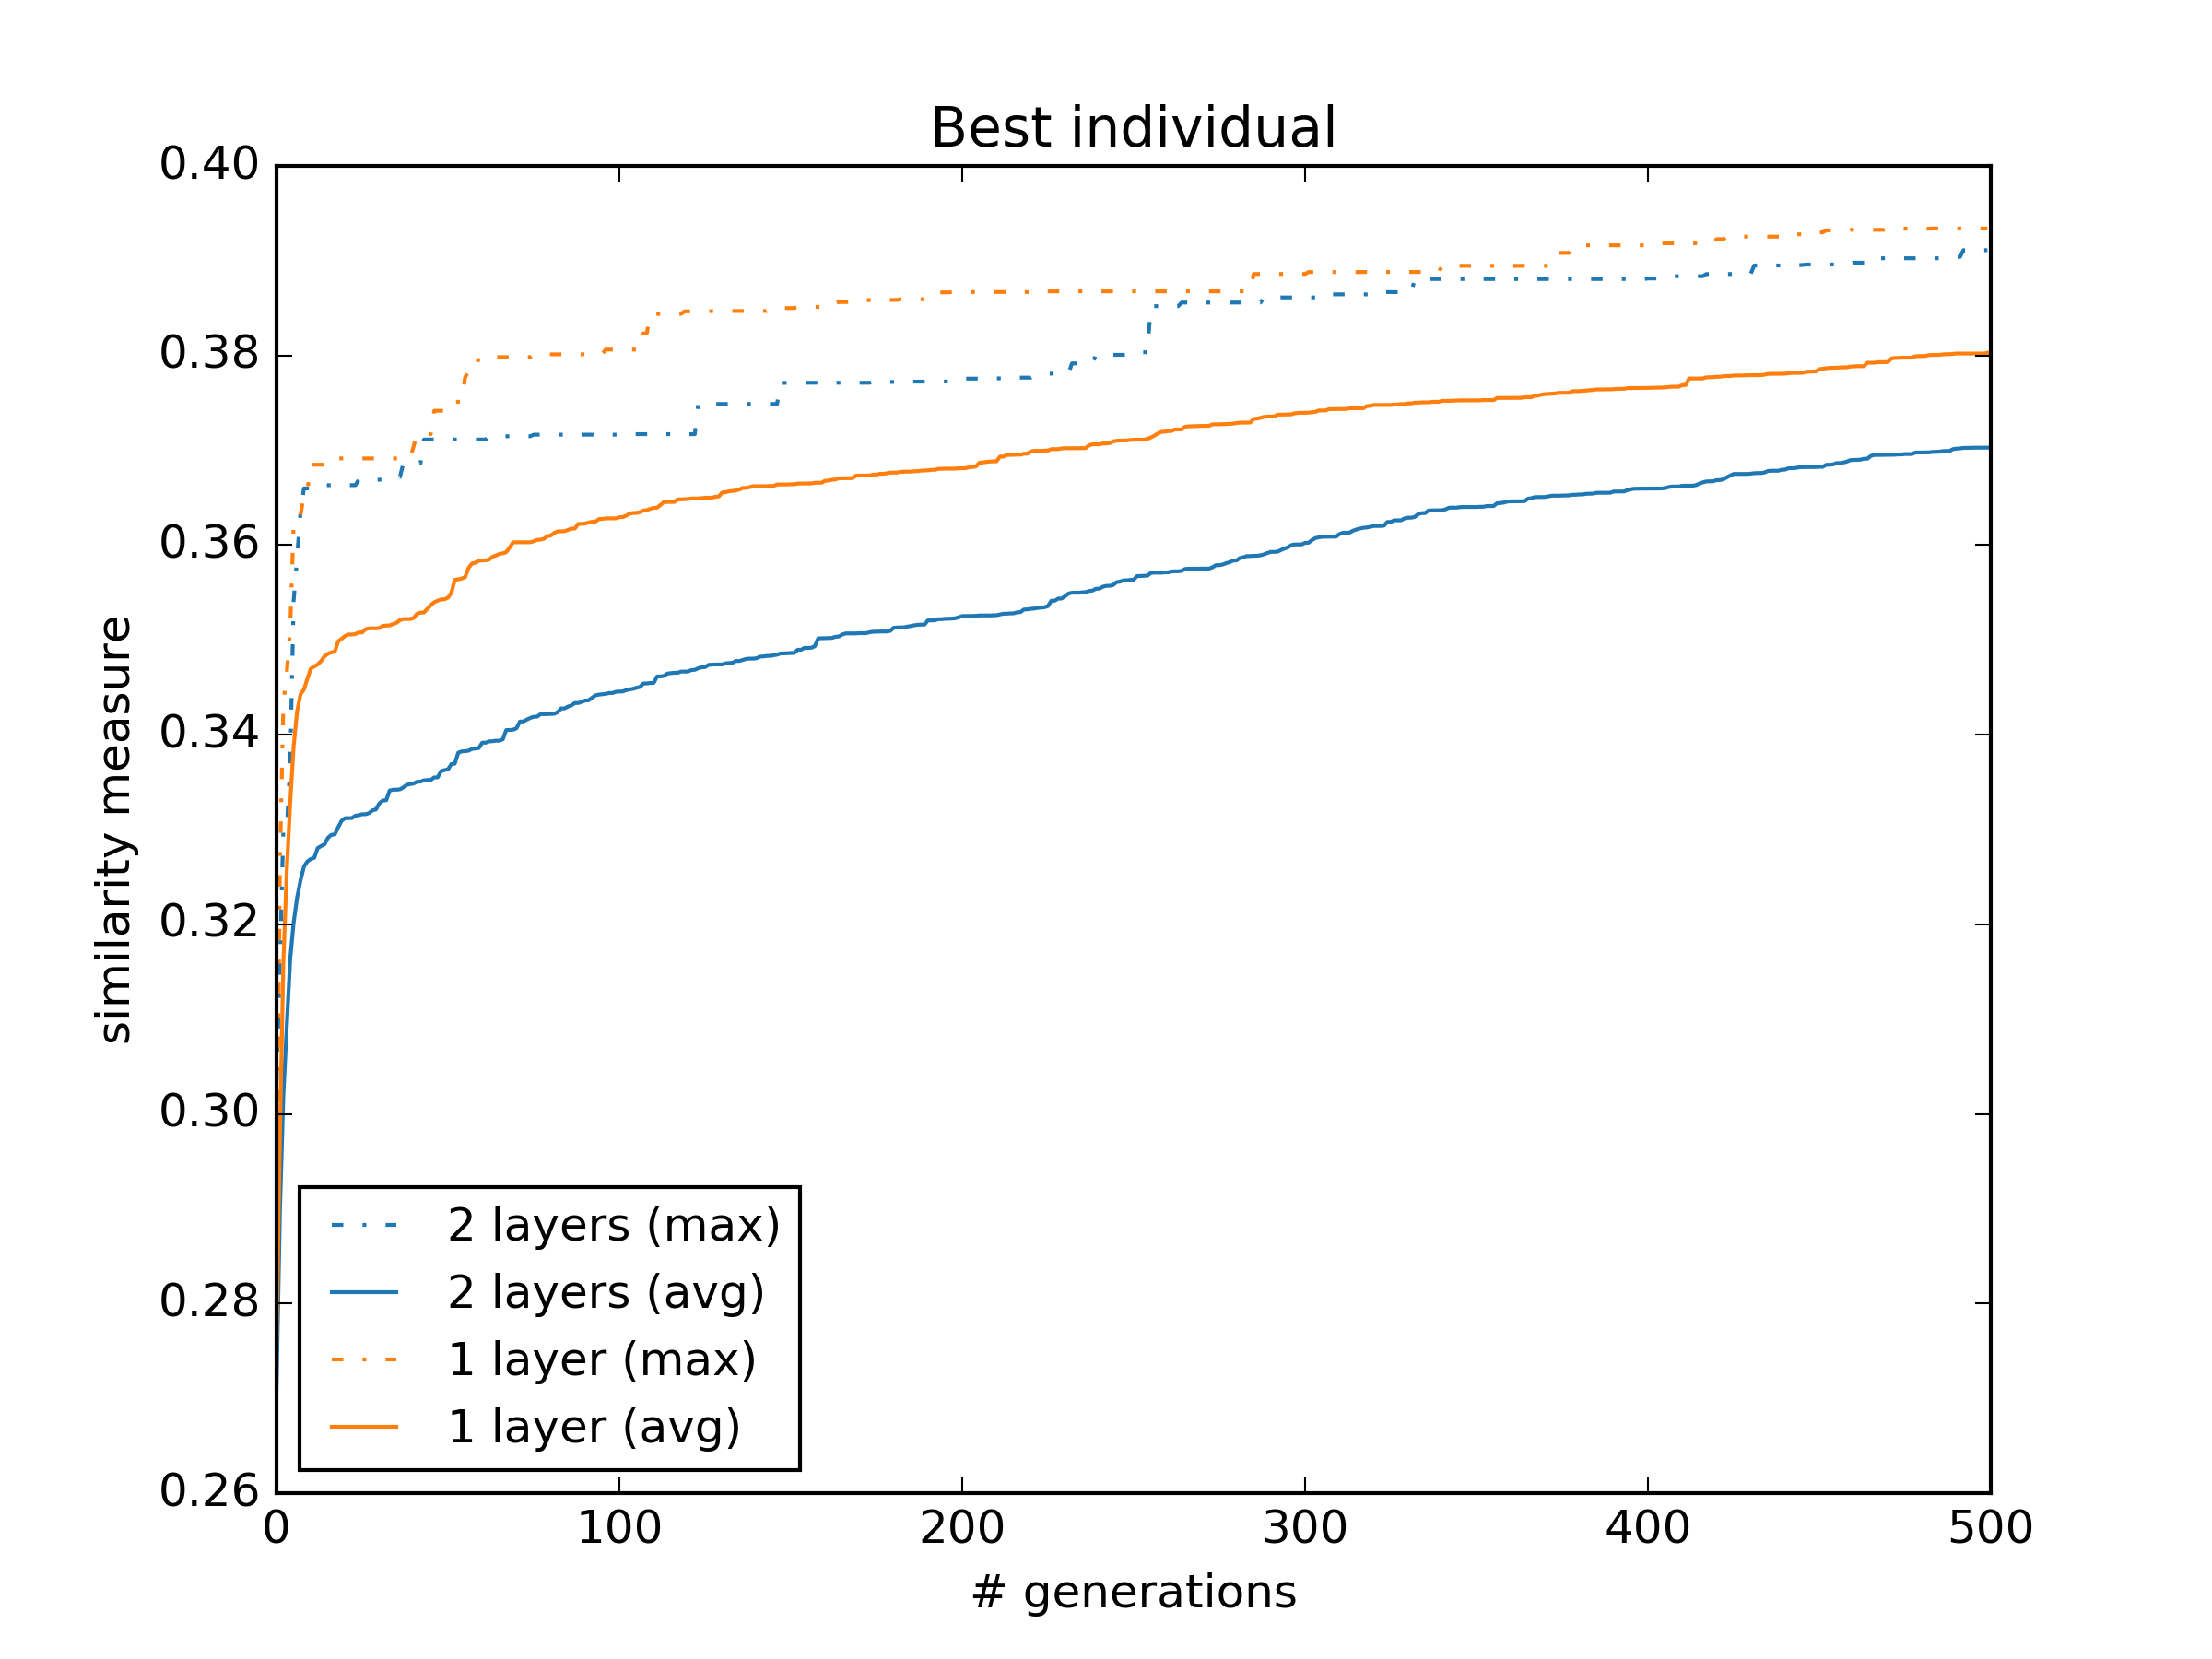
\includegraphics[width=0.99\textwidth]{exp5_avg_max}
    \caption{Aggregated fitness values}
    \label{fig:exp5_avg_max}
\end{figure}

\begin{figure}[h]
    \centering
    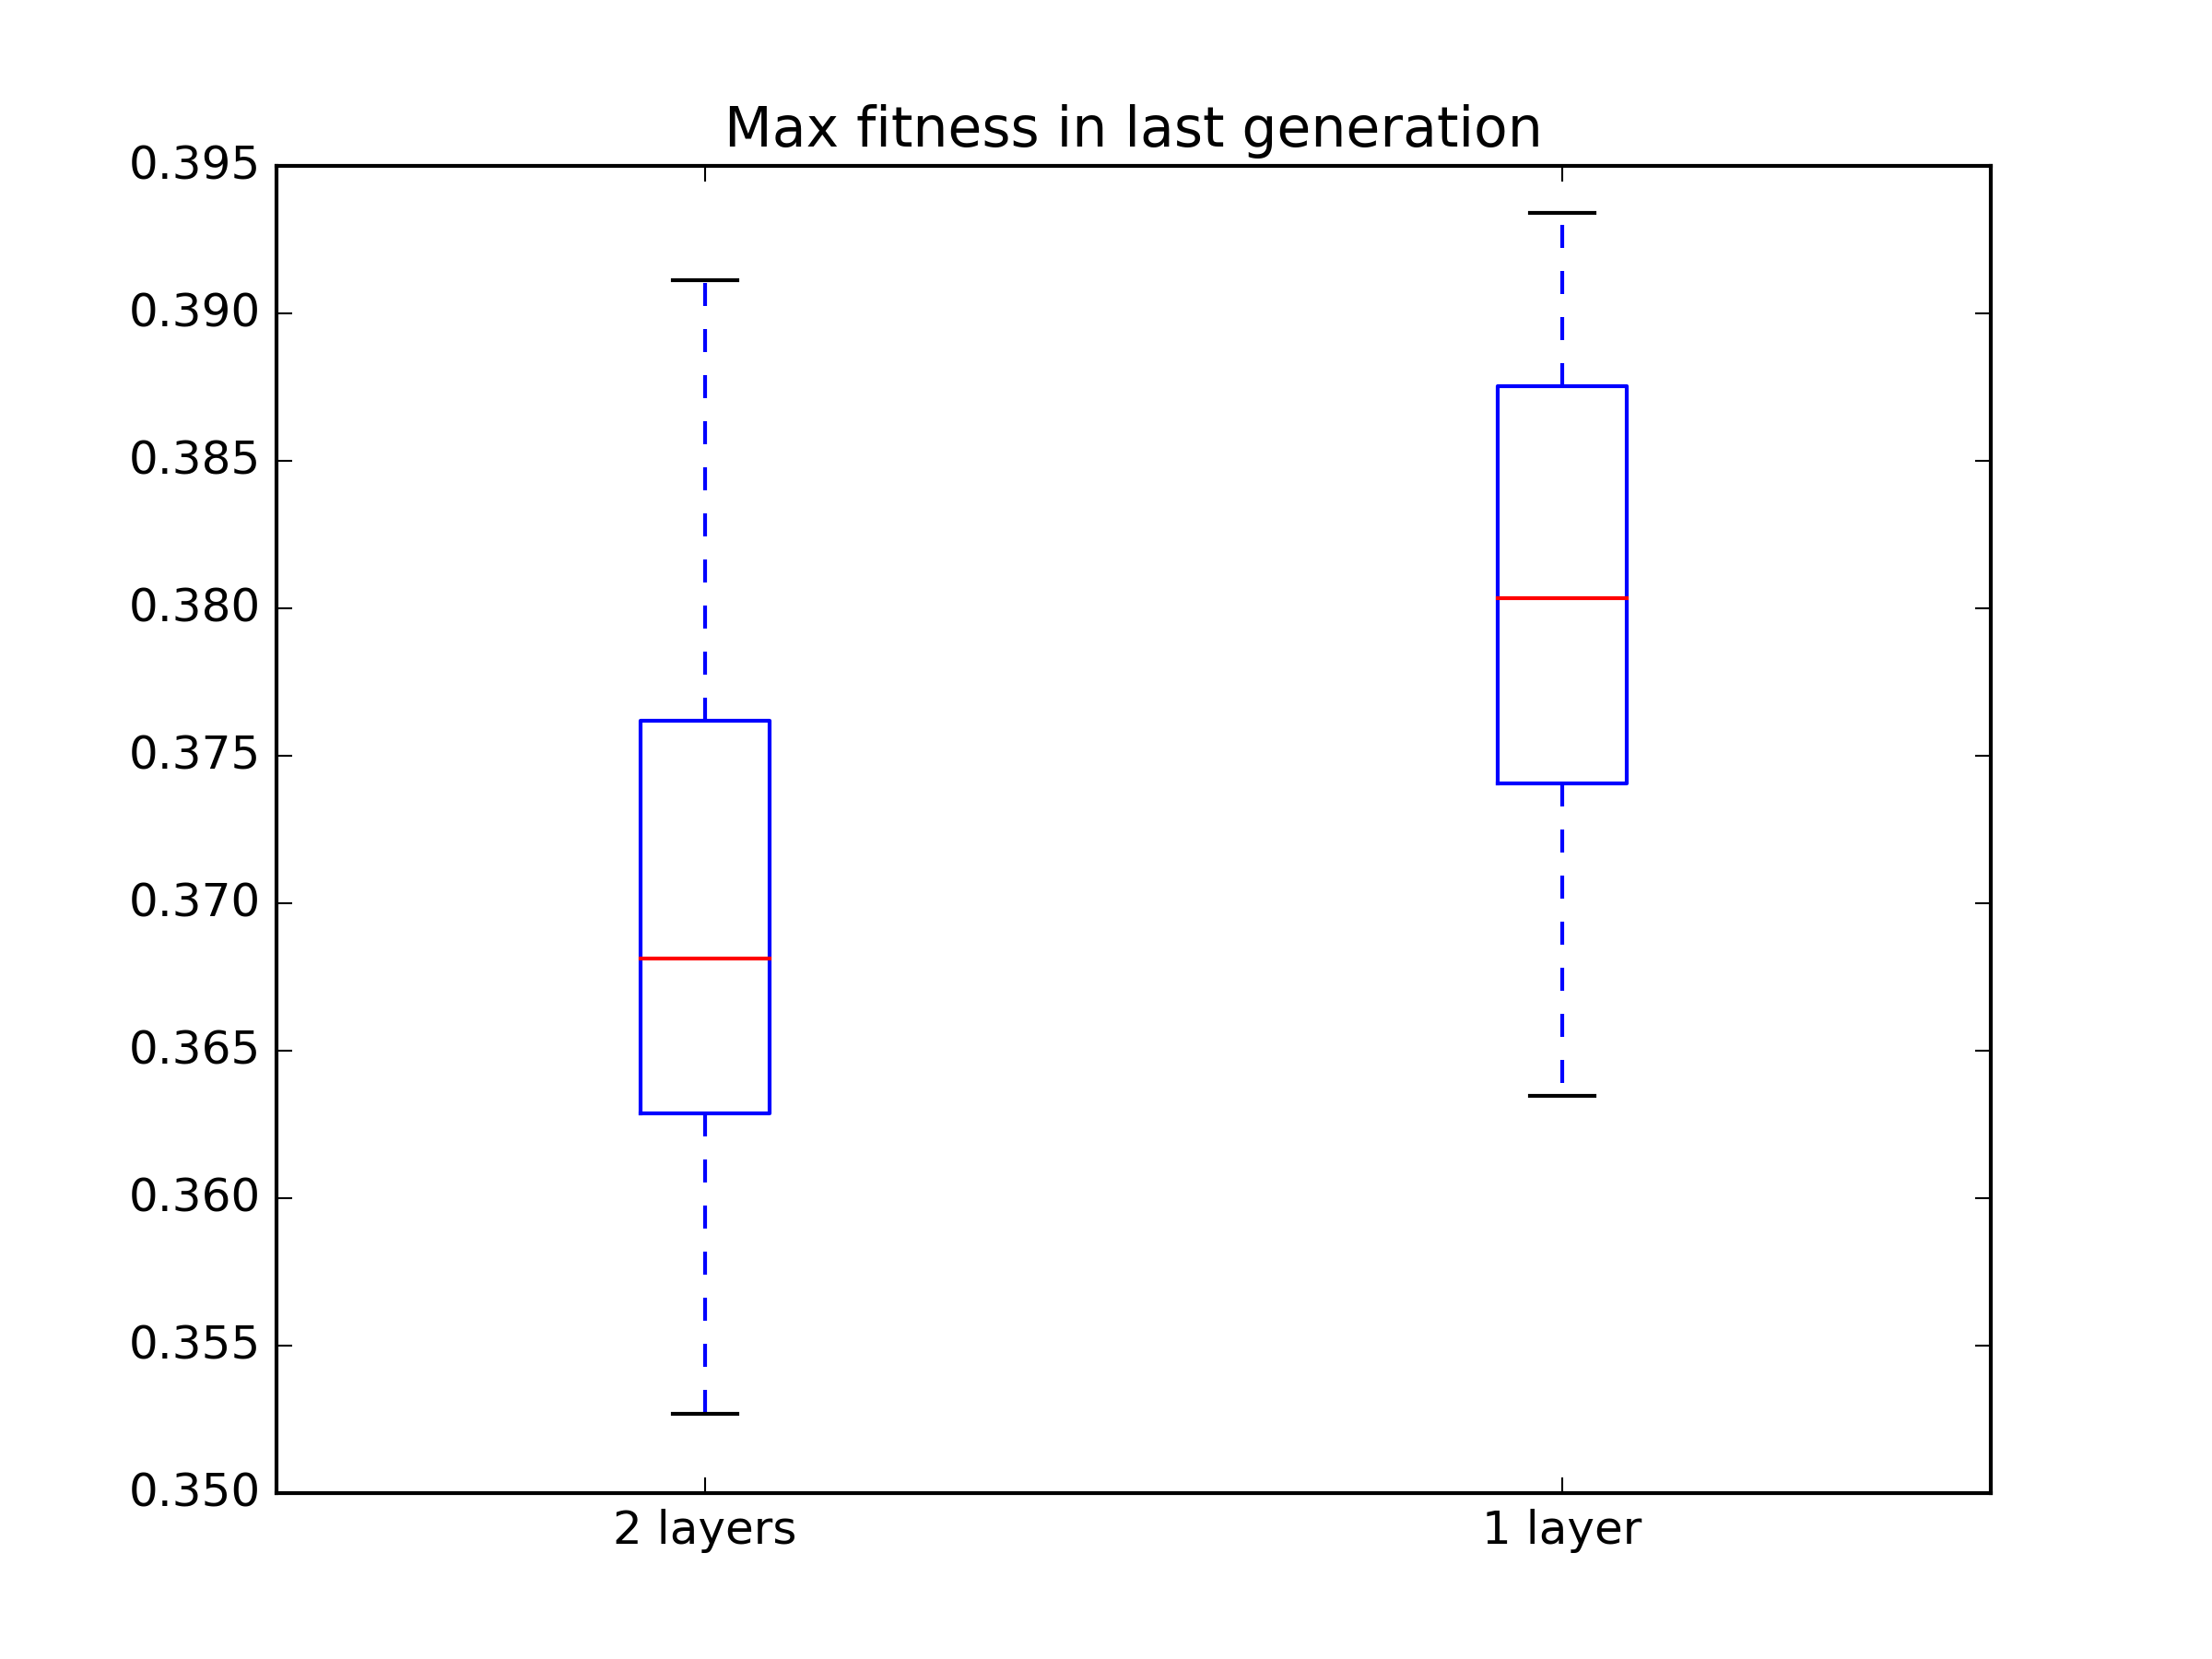
\includegraphics[width=0.99\textwidth]{exp5_box}
    \caption{Box-and-whiskers plot of fitness values in the last generation}
    \label{fig:exp5_box}
\end{figure}


% !TEX encoding = UTF-8 Unicode
%!TEX root = thesis.tex
% !TEX spellcheck = en-US
%%=========================================
\chapter{Conclusion}
\label{chapter:conclusion}

It has been shown that using neuroevolution for finding useful mappings in cross-adaptive audio effects is feasible. This is good because finding these signal mappings by empirical experimentation can be tedious and hard due to the vast number of combinations.

Several fitness functions have been developed and compared. Based on qualitative evaluations, the hybrid variant, that is a combination of local euclidean distance and NSGA-II-inspired multi-objective optimization, has been found to yield the best results. Furthermore, in experiments with high-dimensional spaces, FS-NEAT has been proven to do better than NEAT, because FS-NEAT chooses only a few useful connections rather than a fully connected neural network.

A comprehensive toolkit has been developed during the course of the project. The toolkit includes an interactive visualization tool that makes it possible to evaluate results and understand the neuroevolution process. The toolkit has lots of configuration options, enabling a flexible platform for experimentation. It is open source, has documentation and can be used in future research within the field of cross-adaptive audio effects.

While an evolved cross-adaptive audio effect may perform well on the combination of the input sound and the target sound it was trained on, it is also desirable to be able to apply the effect to other sounds. In particular, this is useful in live performances where audio effects are applied to unseen sound. When training data is scarce, data augmentation can be applied to evolve cross-adaptive audio effects that perform better on unseen sound that deviates from the training sound. Audio effects produced by the toolkit can be used in live performances, thanks to the implementation of audio analysis, audio effects and artificial neural network that can run on live audio streams in Csound.

\section{Future Work}

As stated in the introduction, current research at the Music Technology department at Norwegian University of Science and Technology aims at exploring radically new modes of musical interaction in live music performance. This project is a good start, but there is still a lot to be explored. For example, it would be interesting to try other effects than the five effects used in this project. Also, it does not have to be effects. It can also be sound generators, such as synthesizers or sword sound emulators, with parameters. For example, a foley artist can imitate a sword sound with his mouth, then evolve parameters that make the sword sound generator produce a sound like that. This relates to the work of \cite{cartwright2014}. While their project is based on interactive, iterative refinement through user-provided relevance feedback, neuroevolution can automate that process to save time. That could make foley sound production easier and less time-consuming.

More work can also be done on combining multiple audio effects into one composite audio effect. Experiment 5 performed tests on layers of parallel audio effects, and the results were not better than the best individual effect. However, this does not mean that composite effects are generally bad. There are lots of techniques to be explored that might improve composite effects. For example, one could use Cartesian Genetic Programming (CGP) to automatically evolve the topology of effect networks.

Picbreeder \citep{secretan2008} and Soundbreeder \citep{ye2014} had success with HyperNEAT, which is one variant of NEAT that has not been tried in this project. HyperNEAT might be able to produce better results than NEAT in this project, but probably only in experiments where the input nodes and output nodes have some sort of geometrical meaning \citep{whiteson2013}.

While live mode is implemented and technically works, it has not been tried by music performers yet. There is much work to be done on finding the role of evolved cross-adaptive audio effects in live performances. For example, one has to find out which instruments interact with each other's cross-adaptive effects and which audio effects are musically interesting and appealing. Other potential issues, such as latency and audio feedback, also need to be dealt with.

The author imagines that methods developed in this project could be used for mastering/mixing music and also for novel crossfading in DJ mixing software. However, that would require smart methods for dealing with long sounds (several minutes). This project has only dealt with short sounds (up to 16 seconds) so far. When dealing with longer sounds the author sees two challenges: 1) Computational time and 2) A long sound might have several very different parts, and the evolved neural network might have trouble dealing well with all of them. One possible solution to these challenges is to chop the long sound into a few short audio segments that represent the different parts of the sound well and then run the program on each audio segment. When applying the resulting neural networks on new sounds, the program can automatically fade between the evolved artificial neural networks based on similarity with the various audio segments they were trained on.

% !TEX encoding = UTF-8 Unicode
%!TEX root = thesis.tex
% !TEX spellcheck = en-US
%%=========================================
\addcontentsline{toc}{section}{Acknowledgment}
\section*{Acknowledgment}
I would like to thank the following persons for their great help during \ldots

If the project has been carried out in cooperation with an external partner (e.g., a company), you should acknowledge the contribution and give thanks to the involved persons.

You should also acknowledge the contributions made by your supervisor(s).

\begin{flushright}
O.N.\\[1pc]
(Your initials)
\end{flushright}

%%=========================================
\bibliographystyle{apa}
\addcontentsline{toc}{chapter}{\bibname}
\bibliography{refs}  

%%=========================================
\appendix
%% !TEX encoding = UTF-8 Unicode
%!TEX root = thesis.tex
% !TEX spellcheck = en-US
%%=========================================

\chapter{Acronyms}
\begin{description}
\item[FTA] Fault tree analysis
\item[MTTF] Mean time to failure
\item[RAMS] Reliability, availability, maintainability, and safety
\end{description}
% !TEX encoding = UTF-8 Unicode
%!TEX root = thesis.tex
% !TEX spellcheck = en-US
%%=========================================

\chapter{Open Source Toolkit}
\label{appendix:toolkit}
The toolkit that has been implemented in this project is open source and available at \hfill \break
\url{https://github.com/iver56/cross-adaptive-audio}

This includes software for doing neuroevolution on sounds as well as the software for visualizing the experiments. The readme file includes:

\begin{itemize}
\item Detailed instructions for how to install the project and all dependencies on Windows and Ubuntu
\item User manual with example commands for getting started
\end{itemize}

% !TEX encoding = UTF-8 Unicode
%!TEX root = thesis.tex
% !TEX spellcheck = en-US
%%=========================================

\chapter{Neuroevolution Application Dependencies}
\label{appendix:python_dependencies}

\begin{center}
\begin{longtable}{p{3.3cm} p{13cm}}
\caption[Dependencies]{Dependencies} \label{tab:neuroevolution_dependencies} \\

\hline \multicolumn{1}{l}{\textbf{Name}} & \multicolumn{1}{l}{\textbf{Description}} \\ \hline 
\endfirsthead

\multicolumn{2}{c}
{{\bfseries \tablename\ \thetable{} -- continued from previous page}} \\
\hline \multicolumn{1}{l}{\textbf{Name}} & \multicolumn{1}{l}{\textbf{Description}} \\ \hline 
\endhead

\hline \multicolumn{2}{r}{{Continued on next page}} \\ \hline
\endfoot

\hline \hline
\endlastfoot

\midrule
Jinja2 & A general purpose templating language. Useful for generating csd files that are fed into Csound. \\
\midrule
six, futures & Makes the Python application compatible with both Python 2 and Python 3 \\
\midrule
whichcraft & A tool that can check which programs are installed on the computer. Used for starting Node.js correctly on both Ubuntu and Windows. \\
\midrule
natsort & Natural sorting. Used for showing audio features in the correct order. \\
\midrule
nose & A tool for running all the automated tests in the project \\
\midrule
statistics & A package that can calculate various statistics, for example standard deviation, of data series. \\
\midrule
numpy & A package for scientific computing. Used for computing gradients and euclidean distance. \\
\midrule
matplotlib & A 2D plotting library. Used for creating various plots for this report. \\
\midrule
MultiNEAT & A portable neuroevolution Library written in C++. It has Python bindings. \\
\midrule
Sonic Annotator with Vamp plugin LibXtract & Sonic annotator takes in a set of audio files, runs them through the specified vamp plugin and outputs the results. LibXtract is a library for audio feature extraction. \\
\midrule
Aubio MFCC & A tool that takes in a single audio file and calculates and outputs MFCC coefficients for each frame \\
\midrule
Essentia music extractors & A tool that takes in a single audio file, calculates a large set of audio features and writes the resulting data to a file \\
\midrule
Csound & A sound and music computing system. Csound can be given a piece of Csound code that describes how to process audio, and then Csound processes the audio accordingly. In this project, Csound is used for A) applying audio effects with effect parameters that vary over time and B) calculating audio features. \\

\end{longtable}
\end{center}

% !TEX encoding = UTF-8 Unicode
%!TEX root = thesis.tex
% !TEX spellcheck = en-US
%%=========================================

\chapter{JavaScript libraries in interactive visualization application}
\label{appendix:javascript_dependencies}

\begin{center}
\begin{longtable}{p{3.3cm} p{13cm}}
\caption[JavaScript dependencies]{JavaScript libraries} \label{tab:javascript_dependencies} \\

\hline \multicolumn{1}{l}{\textbf{Name}} & \multicolumn{1}{l}{\textbf{Description}} \\ \hline 
\endfirsthead

\multicolumn{2}{c}%
{{\bfseries \tablename\ \thetable{} -- continued from previous page}} \\
\hline \multicolumn{1}{l}{\textbf{Name}} & \multicolumn{1}{l}{\textbf{Description}} \\ \hline 
\endhead

\hline \multicolumn{2}{r}{{Continued on next page}} \\ \hline
\endfoot

\hline \hline
\endlastfoot

NodeJS & Used for serving the application and pushing results to the application via websockets whenever new data becomes available \\
\hline
AngularJS & Application framework that makes it easy to build Single-Page Applications \\
\hline
Angular-material & User Interface (UI) Component framework. Makes it easy to add UI elements, such as buttons and sliders, that look nice and have great usability. \\
\hline
Color-brewer & Various sets of colors that are useful for visualizing data \\
\hline
Cubism & Time series visualization in the form of horizon charts, which reduce vertical space without losing resolution. This is useful when there are many variables to visualize simultaneously in a limited vertical space. \\
\hline
n3-line-chart & Used for line charts and histograms. Is nicely integrated with AngularJS and features some useful interactions. Depends on D3.js \\
\hline
NVD3 & Chart components for D3.js. Used for creating stacked area chart (species plot) \\
\hline
Debounce, limit & Used for throttling the refresh rate of computationally demanding actions \\
\hline
Sigma & Used for visualizing neural networks. Features zooming, panning and rotating. \\
\hline
Wavesurfer & Works as an audio player that also visualizes the waveform of the sound that is played. The user can click on the waveform to seek to that position. \\
\hline
jQuery & Makes it easier to do Document Object Model (DOM) manipulation \\

\end{longtable}
\end{center}

\end{document}
